%=========================================================
%  Bayesian Fusion Forests --- 25 minute talk
%  Layout follows ISBA2026_v1.tex (metropolis, 16:9).
%
%  Figures are pulled from the manuscript folder and the
%  sticker folder; see \graphicspath below.
%
%  TO SUPPLY (drop into notes/presentations/figures/):
%    figures/VU-logo-CMYK.pdf   -- title page
%    figures/EU-funding.jpg     -- references slide
%  Both are wrapped in \IfFileExists, so the deck compiles
%  without them; they simply do not appear.
%=========================================================
\documentclass[10pt,aspectratio=169]{beamer}

\usetheme{metropolis}
\metroset{sectionpage=none}

\usepackage{amsmath,amssymb,amsfonts}
\usepackage{bm}
\usepackage{booktabs}
\usepackage{tikz}
\usepackage{xcolor}
\usepackage{pgfplots}
\pgfplotsset{compat=1.18}
\usetikzlibrary{arrows.meta, positioning, shapes.geometric, fit, backgrounds,
                decorations.pathreplacing, decorations.markings, calc}

\usepackage{graphicx}
\graphicspath{{figures/}{../general/figures/}{../../sticker/}}
\usepackage{qrcode}

% --- Macros --------------------------------------------------------------
\newcommand{\T}{\mathcal{T}}
\newcommand{\Hh}{\mathcal{H}}
\newcommand{\E}{\mathbb{E}}
\newcommand{\R}{\mathbb{R}}
\newcommand{\N}{\mathcal{N}}
\newcommand{\p}{\mathbb{P}}
\newcommand{\indep}{\perp\!\!\!\perp}

% --- Colour code (used consistently on every slide) ----------------------
\definecolor{myaccent}{HTML}{0077B3}
\definecolor{rctcol}{HTML}{0077B3}     % RCT            (blue)
\definecolor{rwdcol}{HTML}{D95F02}     % RWD            (orange)
\definecolor{taucol}{HTML}{1B9E77}     % treatment effect tau (teal)
\definecolor{confcol}{HTML}{C0392B}    % confounding c  (red)
\definecolor{devcol}{HTML}{7570B3}     % deviation d    (violet)
\definecolor{basecol}{HTML}{555555}    % baseline m0    (grey)

\setbeamercolor{alerted text}{fg=myaccent}
\setbeamercolor{progress bar}{fg=myaccent}
\setbeamercolor{frametitle}{bg=myaccent, fg=white}
\setbeamercolor{normal text}{fg=black!90, bg=white}

% Small inline colour chips for the four model components
\newcommand{\cm}[2]{\textcolor{#1}{#2}}

\title{Bayesian Fusion Forests}
\subtitle{Heterogeneous treatment effects on survival from randomised and
          real-world data}
\date{}
\author{Tijn Jacobs \\
\small joint work with St\'ephanie L.\ van der Pas and Wessel N.\ van Wieringen}
\institute{Vrije Universiteit Amsterdam}

\IfFileExists{figures/VU-logo-CMYK.pdf}{%
  \titlegraphic{%
    \vspace{6.5cm}%
    \hfill\includegraphics[height=1cm]{figures/VU-logo-CMYK.pdf}%
  }}{}

\begin{document}

\maketitle

%=========================================================
\section{Motivation}
%=========================================================

%---------------------------------------------------------
\begin{frame}{Two sources, two weaknesses}
\vspace{0.2cm}
\begin{center}
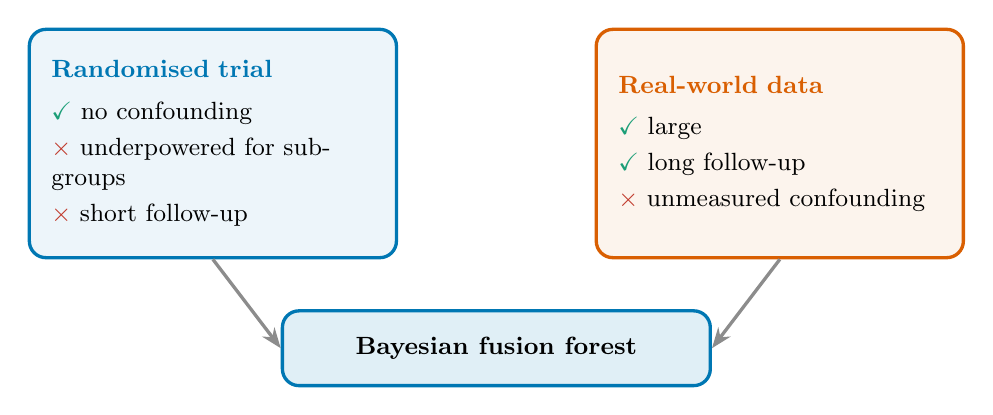
\begin{tikzpicture}[
  src/.style={rounded corners=6pt, draw, very thick, text width=4.1cm,
              minimum height=2.9cm, align=left, inner sep=8pt, font=\small},
  arr/.style={-{Stealth[length=2.6mm]}, very thick, black!45}
]
\node[src, draw=rctcol, fill=rctcol!7] (rct) at (-3.6,0)
  {\textbf{\textcolor{rctcol}{Randomised trial}}\\[4pt]
   \textcolor{taucol}{$\checkmark$} no confounding\\[2pt]
   \textcolor{confcol}{$\times$} underpowered for subgroups\\[2pt]
   \textcolor{confcol}{$\times$} short follow-up};

\node[src, draw=rwdcol, fill=rwdcol!7] (rwd) at (3.6,0)
  {\textbf{\textcolor{rwdcol}{Real-world data}}\\[4pt]
   \textcolor{taucol}{$\checkmark$} large\\[2pt]
   \textcolor{taucol}{$\checkmark$} long follow-up\\[2pt]
   \textcolor{confcol}{$\times$} unmeasured confounding};

\onslide<2->{
\node[rounded corners=6pt, draw=myaccent, very thick, fill=myaccent!12,
      text width=5.2cm, minimum height=0.95cm, align=center,
      font=\small\bfseries] (fuse) at (0,-2.6) {Bayesian fusion forest};
\draw[arr] (rct.south) -- (fuse.west);
\draw[arr] (rwd.south) -- (fuse.east);
}
\end{tikzpicture}
\end{center}

\onslide<3->{
\begin{center}
\alert{Borrow the power, not the bias.}
\end{center}}
\end{frame}

%---------------------------------------------------------
\begin{frame}{Motivating example: antiretroviral therapy for HIV}
\begin{columns}[T,onlytextwidth]
\begin{column}{0.42\textwidth}
\vspace{0.4cm}
\textbf{\textcolor{rctcol}{ACTG 175}} --- trial\\
{\footnotesize $n = 1771$, randomised, $\sim$3 years}

\bigskip

\textbf{\textcolor{rwdcol}{MACS}} --- cohort\\
{\footnotesize $n = 373$, observational, $\sim$25 years,\\ annual visits}

\bigskip\bigskip

Combination therapy vs.\ ZDV monotherapy.

\bigskip

\alert{Who benefits, and by how much?}
\end{column}
\begin{column}{0.56\textwidth}
\centering
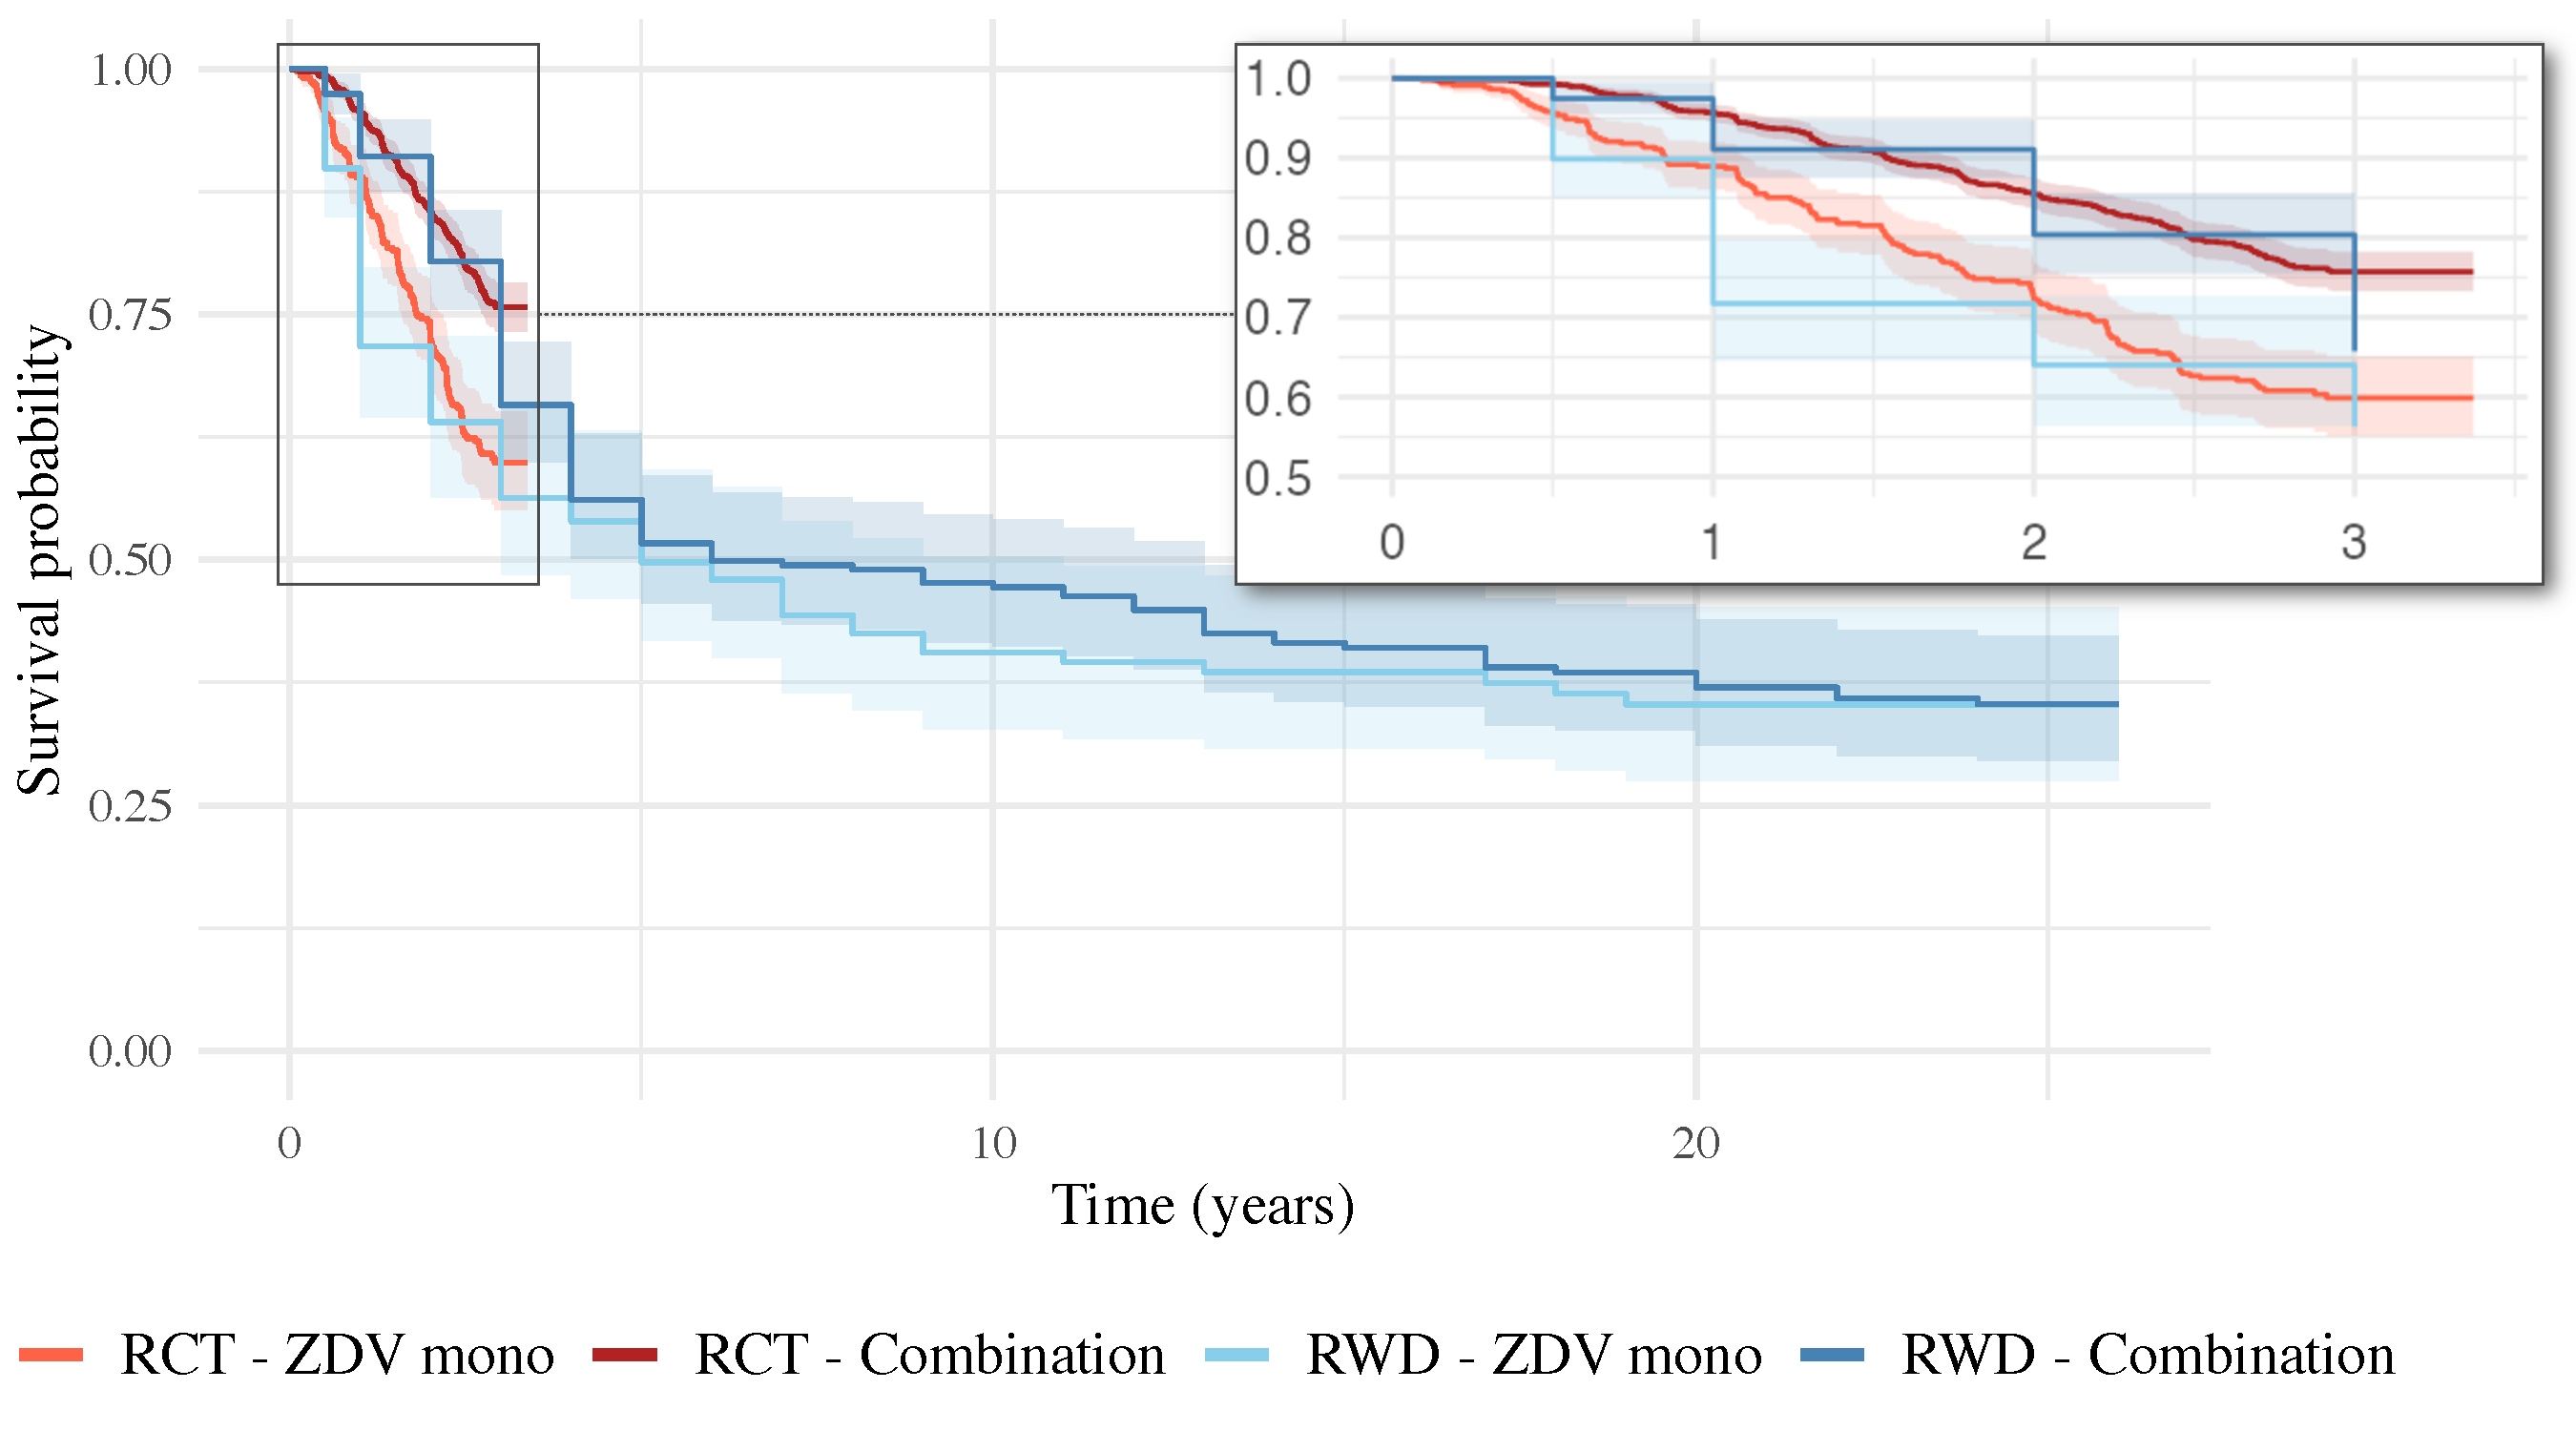
\includegraphics[width=\linewidth]{survival_curves_manuscript.pdf}

{\footnotesize The trial never reaches median survival.}
\end{column}
\end{columns}
\end{frame}

%---------------------------------------------------------
\begin{frame}{Three obstacles}
\vspace{0.3cm}
\begin{center}
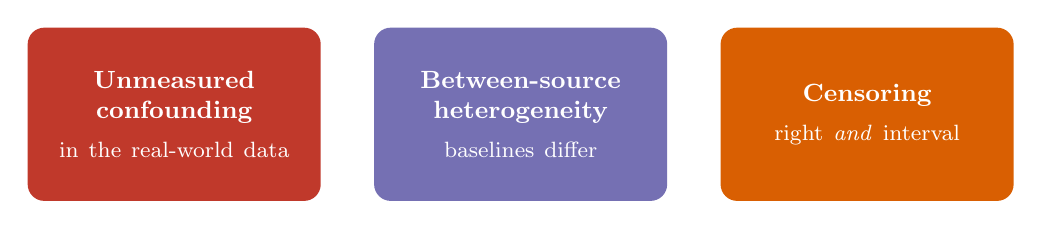
\begin{tikzpicture}[
  ob/.style={rounded corners=6pt, text width=3.3cm, minimum height=2.2cm,
             align=center, text=white, font=\bfseries\small, inner sep=6pt}
]
\node[ob, fill=confcol]  (a) at (-4.4,0)
  {Unmeasured\\ confounding\\[3pt]{\footnotesize\mdseries in the real-world data}};
\node[ob, fill=devcol]   (b) at ( 0.0,0)
  {Between-source\\ heterogeneity\\[3pt]{\footnotesize\mdseries baselines differ}};
\node[ob, fill=rwdcol]   (c) at ( 4.4,0)
  {Censoring\\[3pt]{\footnotesize\mdseries right \emph{and} interval}};
\end{tikzpicture}
\end{center}

\bigskip

\onslide<2->{
\begin{center}
Existing methods handle one or two.\\[4pt]
\alert{We handle all three in one nonparametric model.}
\end{center}}
\end{frame}

%=========================================================
\section{What's new}
%=========================================================

\begin{frame}{Contributions}
\begin{itemize}
  \item \textbf{Swap the assumption.} Drop unconfoundedness in the RWD;
        assume instead that the \emph{treatment effect transports}.
  \vspace{0.55cm}
  \item \textbf{Fusion for survival.} An AFT decomposition that takes
        right- \emph{and} interval-censored outcomes.
  \vspace{0.55cm}
  \item \textbf{The prior does the borrowing.} One tree ensemble per causal
        component, each regularised for its own role.
  \vspace{0.55cm}
  \item \textbf{Errors may differ too.} A hierarchical Dirichlet process
        mixture: source-specific shape, shared components.
\end{itemize}
\end{frame}

%=========================================================
\section{Setup}
%=========================================================

%---------------------------------------------------------
\begin{frame}{What we observe}
\begin{columns}[T,onlytextwidth]
\begin{column}{0.40\textwidth}
\vspace{0.3cm}
Source $S \in \{\textcolor{rwdcol}{0},\textcolor{rctcol}{1}\}$,
treatment $A \in \{0,1\}$, covariates $X \in \R^p$.

\bigskip

Survival time $T$ observed only through a pair $(L, R)$ with $T \in [L, R]$.

\bigskip

\textcolor{rctcol}{Trial:} right-censored.\\[2pt]
\textcolor{rwdcol}{Cohort:} interval-censored.
\end{column}
\begin{column}{0.58\textwidth}
\centering
\vspace{0.2cm}
\resizebox{\linewidth}{!}{%
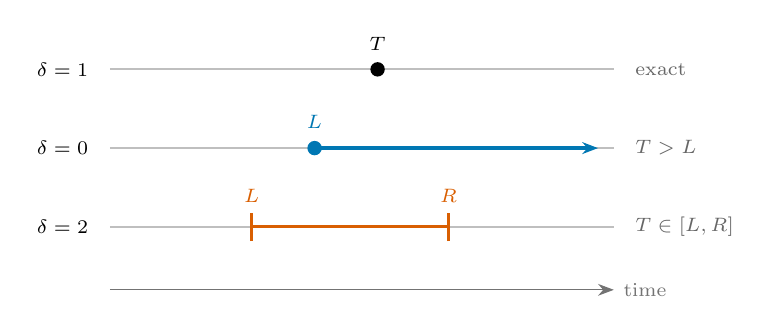
\begin{tikzpicture}[x=1cm, y=1cm]
% three timelines
\foreach \y/\lab in {2/exact, 1/right, 0/interval}{
  \draw[black!25, thick] (0,\y) -- (6.4,\y);
}
% exact
\fill[black] (3.4,2) circle (2.6pt);
\node[left, font=\scriptsize] at (-0.15,2) {$\delta = 1$};
\node[above, font=\scriptsize] at (3.4,2.12) {$T$};
\node[right, font=\scriptsize, text=black!60] at (6.55,2) {exact};
% right censored
\fill[rctcol] (2.6,1) circle (2.6pt);
\draw[-{Stealth[length=2mm]}, very thick, rctcol] (2.6,1) -- (6.2,1);
\node[left, font=\scriptsize] at (-0.15,1) {$\delta = 0$};
\node[above, font=\scriptsize, text=rctcol] at (2.6,1.12) {$L$};
\node[right, font=\scriptsize, text=black!60] at (6.55,1) {$T > L$};
% interval censored
\draw[very thick, rwdcol] (1.8,0) -- (4.3,0);
\draw[very thick, rwdcol] (1.8,-0.18) -- (1.8,0.18);
\draw[very thick, rwdcol] (4.3,-0.18) -- (4.3,0.18);
\node[left, font=\scriptsize] at (-0.15,0) {$\delta = 2$};
\node[above, font=\scriptsize, text=rwdcol] at (1.8,0.18) {$L$};
\node[above, font=\scriptsize, text=rwdcol] at (4.3,0.18) {$R$};
\node[right, font=\scriptsize, text=black!60] at (6.55,0) {$T \in [L,R]$};
% axis
\draw[-{Stealth[length=2mm]}, black!55] (0,-0.8) -- (6.4,-0.8)
  node[right, font=\scriptsize] {time};
\end{tikzpicture}}
\end{column}
\end{columns}
\end{frame}

%---------------------------------------------------------
\begin{frame}{Estimand: the acceleration factor}
\begin{columns}[T,onlytextwidth]
\begin{column}{0.50\textwidth}
\vspace{0.3cm}
CATE on the log-time scale:
\[
\textcolor{taucol}{\tau(x)} \;=\; \E\bigl[\log T(1) - \log T(0) \mid X = x\bigr].
\]

\bigskip

On the time scale,
\[
T(1) \mid X = x \;\overset{d}{=}\; e^{\textcolor{taucol}{\tau(x)}}\, T(0) \mid X = x.
\]

\bigskip

\begin{itemize}
  \item Treatment \emph{stretches the clock}.
  \item Collapsible; keeps its causal meaning where the hazard ratio does not.
\end{itemize}
\end{column}
\begin{column}{0.48\textwidth}
\centering
\vspace{0.2cm}
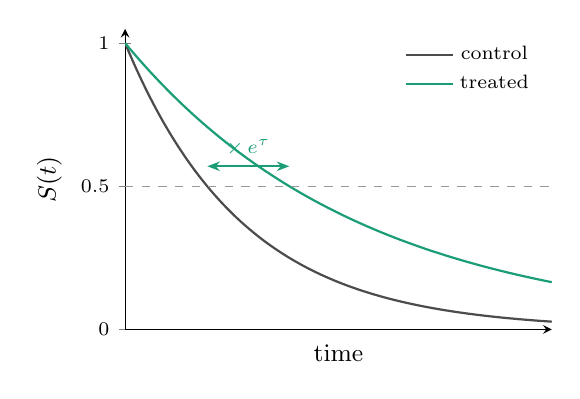
\begin{tikzpicture}
\begin{axis}[
  width=7.0cm, height=5.4cm,
  xlabel={time}, ylabel={$S(t)$},
  xmin=0, xmax=12, ymin=0, ymax=1.05,
  xtick=\empty, ytick={0,0.5,1},
  legend style={font=\scriptsize, draw=none, fill=none,
                at={(0.98,0.98)}, anchor=north east},
  axis lines=left,
  tick label style={font=\scriptsize},
  label style={font=\small},
]
\addplot[domain=0:12, samples=200, thick, black!70]  {exp(-0.30*x)};
\addlegendentry{control}
\addplot[domain=0:12, samples=200, thick, taucol]    {exp(-0.15*x)};
\addlegendentry{treated}
\draw[dashed, black!40] (axis cs:0,0.5) -- (axis cs:12,0.5);
\draw[{Stealth[length=1.6mm]}-{Stealth[length=1.6mm]}, thick, taucol]
  (axis cs:2.31,0.57) -- (axis cs:4.62,0.57)
  node[midway, above, font=\scriptsize, text=taucol] {$\times\, e^{\tau}$};
\end{axis}
\end{tikzpicture}

{\footnotesize $e^{\tau(x)} = 2 \Rightarrow$ median survival doubles.}
\end{column}
\end{columns}
\end{frame}

%---------------------------------------------------------
\begin{frame}{The assumption we drop, and the one we keep}
\begin{columns}[T,onlytextwidth]
\begin{column}{0.48\textwidth}
\centering
\textbf{\textcolor{rctcol}{Trial}}\\[0.4cm]
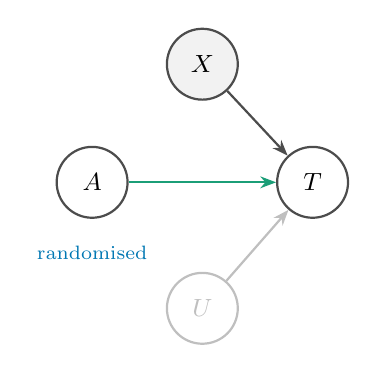
\begin{tikzpicture}[
  nd/.style={circle, draw=black!70, thick, minimum size=9mm, font=\small},
  arr/.style={-{Stealth[length=2mm]}, thick, black!70}
]
\node[nd, fill=black!5] (X) at (0,1.5)   {$X$};
\node[nd] (A) at (-1.4,0) {$A$};
\node[nd] (T) at (1.4,0)  {$T$};
\node[nd, draw=black!25, text=black!25] (U) at (0,-1.6) {$U$};
\draw[arr] (X) -- (T);
\draw[arr, taucol] (A) -- (T);
\draw[arr, black!25] (U) -- (T);
\node[font=\scriptsize, text=rctcol] at (-1.4,-0.9) {randomised};
\end{tikzpicture}

\bigskip
{\footnotesize No arrow into $A$: unconfounded by design.}
\end{column}
\begin{column}{0.48\textwidth}
\centering
\textbf{\textcolor{rwdcol}{Real-world data}}\\[0.4cm]
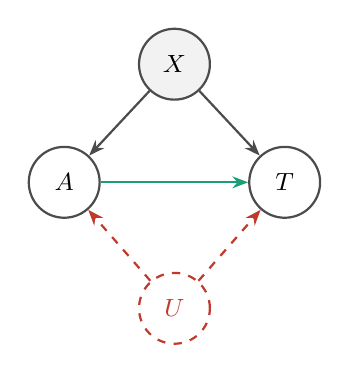
\begin{tikzpicture}[
  nd/.style={circle, draw=black!70, thick, minimum size=9mm, font=\small},
  arr/.style={-{Stealth[length=2mm]}, thick, black!70}
]
\node[nd, fill=black!5] (X) at (0,1.5)   {$X$};
\node[nd] (A) at (-1.4,0) {$A$};
\node[nd] (T) at (1.4,0)  {$T$};
\node[nd, draw=confcol, text=confcol, dashed] (U) at (0,-1.6) {$U$};
\draw[arr] (X) -- (A);
\draw[arr] (X) -- (T);
\draw[arr, taucol] (A) -- (T);
\draw[arr, confcol, dashed] (U) -- (A);
\draw[arr, confcol, dashed] (U) -- (T);
\end{tikzpicture}

\bigskip
{\footnotesize \textcolor{confcol}{$U$ unmeasured: back-door path stays open.}}
\end{column}
\end{columns}

\bigskip

\onslide<2->{
\begin{center}
\alert{Transportability.}\;
$\textcolor{taucol}{\tau(x)}$ is the same in both sources.
\end{center}}
\end{frame}

%=========================================================
\section{The model}
%=========================================================

%---------------------------------------------------------
\begin{frame}{One decomposition, four functions}
\vspace{-0.1cm}
\[
\log T \;=\;
\underbrace{\cm{basecol}{m_0^{\mathrm{sh}}(X)}}_{\text{shared baseline}}
\;+\;
(1-S)\,\underbrace{\cm{devcol}{d(X)}}_{\text{source deviation}}
\;+\;
A\,\underbrace{\cm{taucol}{\tau(X)}}_{\text{treatment effect}}
\;+\;
(1-S)\,A\,\underbrace{\cm{confcol}{c(X)}}_{\text{confounding}}
\;+\;\varepsilon
\]

\vspace{0.3cm}

\begin{center}
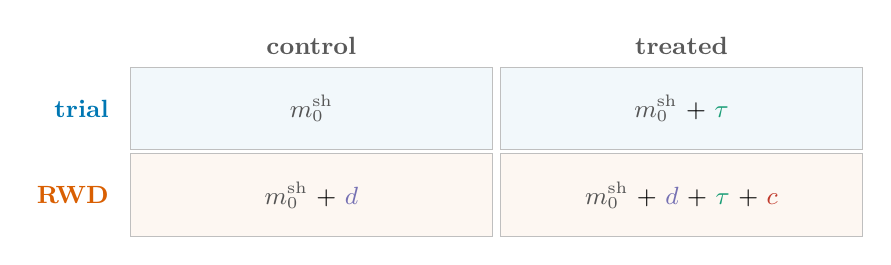
\begin{tikzpicture}[
  cell/.style={draw=black!25, minimum width=4.6cm, minimum height=1.05cm,
               font=\small, align=center},
  hd/.style={font=\small\bfseries, text=black!65}
]
\node[hd] at (0,1.05) {control};
\node[hd] at (4.7,1.05) {treated};
\node[hd, anchor=east, text=rctcol] at (-2.45,0.25) {trial};
\node[hd, anchor=east, text=rwdcol] at (-2.45,-0.85) {RWD};

\node[cell, fill=rctcol!5] at (0,0.25)
  {\cm{basecol}{$m_0^{\mathrm{sh}}$}};
\node[cell, fill=rctcol!5] at (4.7,0.25)
  {\cm{basecol}{$m_0^{\mathrm{sh}}$} $+$ \cm{taucol}{$\tau$}};
\node[cell, fill=rwdcol!5] at (0,-0.85)
  {\cm{basecol}{$m_0^{\mathrm{sh}}$} $+$ \cm{devcol}{$d$}};
\node[cell, fill=rwdcol!5] at (4.7,-0.85)
  {\cm{basecol}{$m_0^{\mathrm{sh}}$} $+$ \cm{devcol}{$d$} $+$
   \cm{taucol}{$\tau$} $+$ \cm{confcol}{$c$}};
\end{tikzpicture}
\end{center}

\vspace{0.2cm}
{\footnotesize The confounding function \cm{confcol}{$c$} is the gap between the
real-world contrast and the causal effect.}
\end{frame}

%---------------------------------------------------------
\begin{frame}{Identification: who pins down what}
\vspace{0.3cm}
\begin{center}
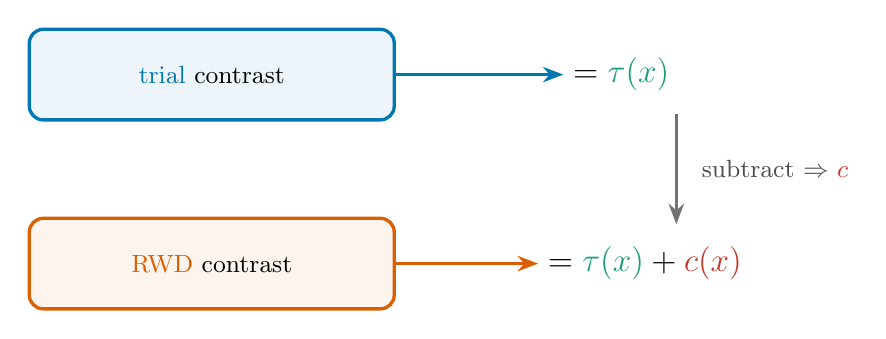
\begin{tikzpicture}[
  box/.style={rounded corners=5pt, draw, very thick, text width=4.4cm,
              minimum height=1.15cm, align=center, font=\small},
  arr/.style={-{Stealth[length=2.6mm]}, very thick}
]
\node[box, draw=rctcol, fill=rctcol!7] (r1) at (-3.6,1.4)
  {\textcolor{rctcol}{trial} contrast};
\node[box, draw=rwdcol, fill=rwdcol!7] (r0) at (-3.6,-1.0)
  {\textcolor{rwdcol}{RWD} contrast};

\node[font=\large] (t1) at (1.6,1.4) {$= \cm{taucol}{\tau(x)}$};
\node[font=\large] (t0) at (1.9,-1.0)
  {$= \cm{taucol}{\tau(x)} + \cm{confcol}{c(x)}$};

\draw[arr, rctcol] (r1) -- (t1);
\draw[arr, rwdcol] (r0) -- (t0);

\onslide<2->{
\draw[arr, black!55] (2.3,0.9) -- (2.3,-0.5);
\node[right, font=\small, text=black!70] at (2.5,0.2)
  {subtract $\Rightarrow$ \cm{confcol}{$c$}};}
\end{tikzpicture}
\end{center}

\bigskip

\onslide<3->{
\begin{center}
\alert{The RWD alone identifies only the sum.}\\[3pt]
{\footnotesize Not a sample-size problem --- no amount of real-world data resolves it.}
\end{center}}
\end{frame}

%---------------------------------------------------------
\begin{frame}{BART in one slide}
\begin{center}
\begin{minipage}[c]{0.38\linewidth}
  \centering
  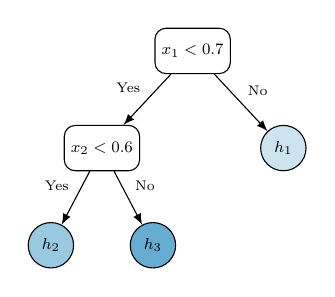
\begin{tikzpicture}[
        scale=0.72, transform shape,
        box/.style={rectangle, draw, rounded corners, align=center,
                    minimum height=8mm, minimum width=13mm, font=\footnotesize},
        leaf/.style={circle, draw, align=center, minimum size=8mm,
                     font=\footnotesize},
        line/.style={-latex}
    ]
    \node [box] (root) {$x_1 < 0.7$};
    \node [box, below=0.9cm of root, xshift=-1.6cm] (left) {$x_2 < 0.6$};
    \node [leaf, fill=myaccent!20, below=0.9cm of root, xshift=1.6cm] (h1) {$h_1$};
    \node [leaf, fill=myaccent!40, below=0.9cm of left, xshift=-0.9cm] (h2) {$h_2$};
    \node [leaf, fill=myaccent!60, below=0.9cm of left, xshift=0.9cm] (h3) {$h_3$};
    \draw[line] (root) -- (left) node[midway, above left, font=\scriptsize] {Yes};
    \draw[line] (root) -- (h1) node[midway, above right, font=\scriptsize] {No};
    \draw[line] (left) -- (h2) node[midway, above left, font=\scriptsize] {Yes};
    \draw[line] (left) -- (h3) node[midway, above right, font=\scriptsize] {No};
  \end{tikzpicture}
\end{minipage}\hfill
\begin{minipage}[c]{0.08\linewidth}
  \centering
  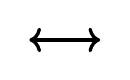
\begin{tikzpicture}\draw[<->, very thick] (0,0) -- (0.9,0);\end{tikzpicture}
\end{minipage}\hfill
\begin{minipage}[c]{0.38\linewidth}
  \centering
  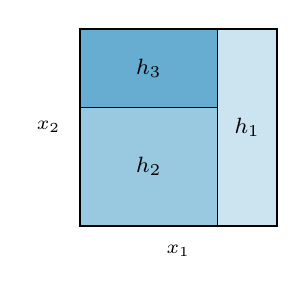
\begin{tikzpicture}[scale=2.5]
    \fill[myaccent!20] (0.7, 0) rectangle (1, 1);
    \fill[myaccent!40] (0, 0)   rectangle (0.7, 0.6);
    \fill[myaccent!60] (0, 0.6) rectangle (0.7, 1);
    \draw[thick] (0, 0) rectangle (1, 1);
    \draw[thin] (0.7, 0) -- (0.7, 1);
    \draw[thin] (0, 0.6) -- (0.7, 0.6);
    \node[below, font=\scriptsize] at (0.5, -0.05) {$x_1$};
    \node[left, font=\scriptsize] at (-0.05, 0.5) {$x_2$};
    \node[font=\footnotesize] at (0.85, 0.5) {$h_1$};
    \node[font=\footnotesize] at (0.35, 0.3) {$h_2$};
    \node[font=\footnotesize] at (0.35, 0.8) {$h_3$};
  \end{tikzpicture}
\end{minipage}
\end{center}

\vspace{0.2em}

\[
f(x) \;=\; \sum_{j=1}^{J} g(x;\, \T_j, \Hh_j)
\]

\begin{center}
{\small A sum of $J$ shallow trees. Depth-penalised prior
$\alpha(1+d)^{-\beta}$; Gaussian step heights of scale $k$.}
\end{center}
\end{frame}

%---------------------------------------------------------
\begin{frame}{One forest per component --- and a ladder of regularisation}
\vspace{0.2cm}
\begin{center}
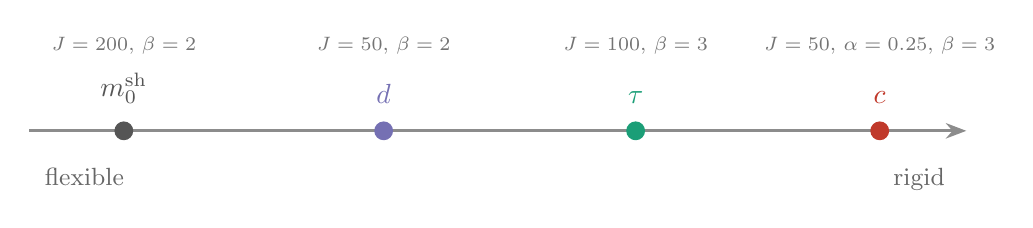
\begin{tikzpicture}[x=1cm, y=1cm]
% axis
\draw[-{Stealth[length=2.6mm]}, very thick, black!45] (-0.3,0) -- (11.6,0);
\node[below, font=\small, text=black!60] at (0.4,-0.35) {flexible};
\node[below, font=\small, text=black!60] at (11.0,-0.35) {rigid};

\foreach \x/\col/\name/\spec in {
  0.9/basecol/{$m_0^{\mathrm{sh}}$}/{$J=200$, $\beta=2$},
  4.2/devcol/{$d$}/{$J=50$, $\beta=2$},
  7.4/taucol/{$\tau$}/{$J=100$, $\beta=3$},
  10.5/confcol/{$c$}/{$J=50$, $\alpha=0.25$, $\beta=3$}
}{
  \fill[\col] (\x,0) circle (3.4pt);
  \node[above, font=\normalsize, text=\col] at (\x,0.22) {\name};
  \node[above, font=\scriptsize, text=black!55] at (\x,0.85) {\spec};
}
\end{tikzpicture}
\end{center}

\bigskip

\begin{itemize}\setlength\itemsep{0.25em}
  \item \cm{basecol}{$m_0^{\mathrm{sh}}$} enters every observation $\Rightarrow$ let it be complex.
  \item \cm{devcol}{$d$} is mean-zero $\Rightarrow$ the prior \emph{centres on equality} of the two baselines.
  \item \cm{taucol}{$\tau$} shrunk towards a homogeneous effect.
  \item \cm{confcol}{$c$} shrunk towards a constant bias --- it comes from what we did not measure.
\end{itemize}
\end{frame}

%---------------------------------------------------------
\begin{frame}{Borrowing is a prior, not a switch}
\begin{columns}[T,onlytextwidth]
\begin{column}{0.46\textwidth}
\vspace{0.4cm}
\[
m_0(X, S) \;=\; \cm{basecol}{m_0^{\mathrm{sh}}(X)} \;+\; (1-S)\,\cm{devcol}{d(X)}
\]

\bigskip

The deviation scale $k_d$ tunes how far the two baselines may drift apart.

\bigskip

\begin{itemize}
  \item $k_d \to 0$: full pooling.
  \item $k_d$ large: two separate baselines.
\end{itemize}

\bigskip
{\footnotesize A meta-analytic-predictive prior on the prognostic surface.}
\end{column}
\begin{column}{0.52\textwidth}
\centering
\vspace{0.1cm}
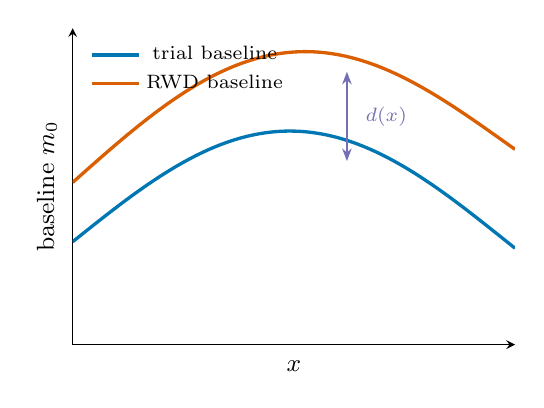
\begin{tikzpicture}
\begin{axis}[
  width=7.2cm, height=5.6cm,
  xlabel={$x$}, ylabel={baseline $m_0$},
  xmin=0, xmax=1, ymin=-1.6, ymax=2.4,
  xtick=\empty, ytick=\empty, axis lines=left,
  label style={font=\small},
  legend style={font=\scriptsize, draw=none, fill=none,
                at={(0.02,0.98)}, anchor=north west},
]
\addplot[domain=0:1, samples=100, very thick, rctcol]
  {1.4*sin(deg(3.2*x)) - 0.3};
\addlegendentry{trial baseline}
\addplot[domain=0:1, samples=100, very thick, rwdcol]
  {1.4*sin(deg(3.2*x)) - 0.3 + 0.75 + 0.5*x};
\addlegendentry{RWD baseline}
\draw[{Stealth[length=1.6mm]}-{Stealth[length=1.6mm]}, thick, devcol]
  (axis cs:0.62,0.72) -- (axis cs:0.62,1.85);
\node[right, font=\scriptsize, text=devcol] at (axis cs:0.64,1.28) {$d(x)$};
\end{axis}
\end{tikzpicture}
\end{column}
\end{columns}
\end{frame}

%---------------------------------------------------------
\begin{frame}{The errors may differ too}
\begin{columns}[T,onlytextwidth]
\begin{column}{0.42\textwidth}
\vspace{0.4cm}
Protocol, follow-up quality and extreme outcomes differ between sources.

\bigskip

Hierarchical Dirichlet process mixture:
\[
G^* \sim \mathrm{DP}(\gamma, H), \quad
G_s^* \sim \mathrm{DP}(M_s, G^*).
\]

\bigskip

\begin{itemize}
  \item \alert{Shared} mixture components.
  \item \alert{Source-specific} weights.
  \item Centred, so $\E[\varepsilon \mid S] = 0$.
\end{itemize}
\end{column}
\begin{column}{0.56\textwidth}
\centering
\vspace{0.1cm}
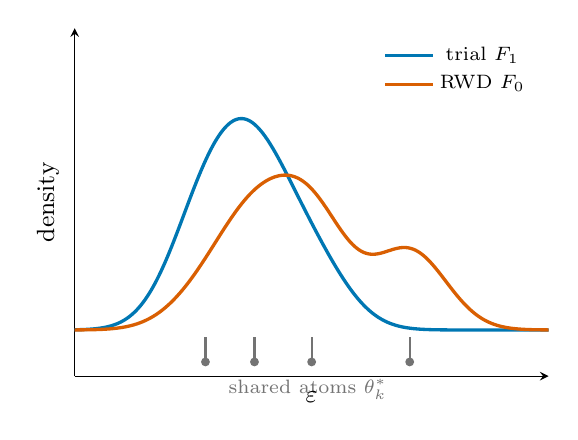
\begin{tikzpicture}
\begin{axis}[
  width=7.6cm, height=6.0cm,
  xlabel={$\varepsilon$}, ylabel={density},
  xmin=-2.2, xmax=3.6, ymin=-0.13, ymax=0.85,
  ytick=\empty, xtick=\empty, axis lines=left, clip=false,
  legend style={font=\scriptsize, draw=none, fill=none,
                at={(0.98,0.98)}, anchor=north east},
  label style={font=\small},
]
% shared atoms at -0.6, 0.0, 0.7, 1.9 ; common scale 0.45
\addplot[domain=-2.2:3.6, samples=250, very thick, rctcol]
  {0.35*0.8865*exp(-(x+0.6)^2/0.405)
 + 0.45*0.8865*exp(-(x)^2/0.405)
 + 0.20*0.8865*exp(-(x-0.7)^2/0.405)};
\addlegendentry{trial $F_1$}
\addplot[domain=-2.2:3.6, samples=250, very thick, rwdcol]
  {0.10*0.8865*exp(-(x+0.6)^2/0.405)
 + 0.30*0.8865*exp(-(x)^2/0.405)
 + 0.35*0.8865*exp(-(x-0.7)^2/0.405)
 + 0.25*0.8865*exp(-(x-1.9)^2/0.405)};
\addlegendentry{RWD $F_0$}
% shared atoms as stems below the axis
% (written out rather than \foreach: \foreach breaks "axis cs:" parsing)
\draw[black!55, thick] (axis cs:-0.6,-0.02) -- (axis cs:-0.6,-0.09);
\fill[black!55] (axis cs:-0.6,-0.09) circle (1.6pt);
\draw[black!55, thick] (axis cs:0.0,-0.02) -- (axis cs:0.0,-0.09);
\fill[black!55] (axis cs:0.0,-0.09) circle (1.6pt);
\draw[black!55, thick] (axis cs:0.7,-0.02) -- (axis cs:0.7,-0.09);
\fill[black!55] (axis cs:0.7,-0.09) circle (1.6pt);
\draw[black!55, thick] (axis cs:1.9,-0.02) -- (axis cs:1.9,-0.09);
\fill[black!55] (axis cs:1.9,-0.09) circle (1.6pt);
\node[font=\scriptsize, text=black!55, anchor=north]
  at (axis cs:0.65,-0.11) {shared atoms $\theta_k^*$};
\end{axis}
\end{tikzpicture}
\end{column}
\end{columns}
\end{frame}

%---------------------------------------------------------
\begin{frame}{Posterior inference}
\vspace{0.3cm}
\begin{center}
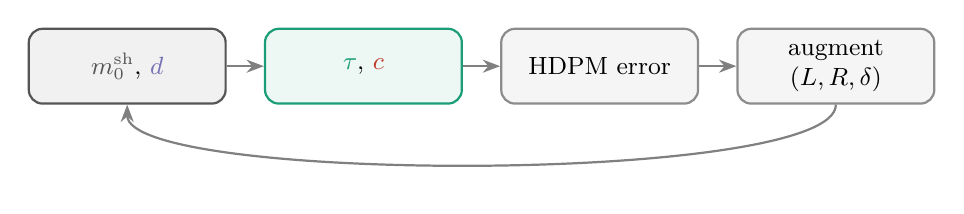
\begin{tikzpicture}[
  blk/.style={rounded corners=5pt, draw, thick, minimum width=2.5cm,
              minimum height=0.95cm, align=center, font=\small},
  arr/.style={-{Stealth[length=2.2mm]}, thick, black!50}
]
\node[blk, draw=basecol, fill=basecol!8] (m) at (-4.5,0) {\cm{basecol}{$m_0^{\mathrm{sh}}$}, \cm{devcol}{$d$}};
\node[blk, draw=taucol, fill=taucol!8]   (t) at (-1.5,0) {\cm{taucol}{$\tau$}, \cm{confcol}{$c$}};
\node[blk, draw=black!45, fill=black!4]  (e) at ( 1.5,0) {HDPM error};
\node[blk, draw=black!45, fill=black!4]  (d) at ( 4.5,0) {augment\\ $(L,R,\delta)$};
\draw[arr] (m) -- (t);
\draw[arr] (t) -- (e);
\draw[arr] (e) -- (d);
\draw[arr] (d.south) .. controls (4.5,-1.5) and (-4.5,-1.5) .. (m.south);
\end{tikzpicture}
\end{center}

\bigskip

\begin{itemize}
  \item Blocked Gibbs: each forest updates against its partial residual, so
        every step is a \emph{standard} BART update.
  \item Censored times are latent variables (Tanner \& Wong, 1987) --- this is
        where interval censoring enters, not the identification argument.
  \item Average effects by a hierarchical Bayesian bootstrap over the target
        covariate distribution.
\end{itemize}
\end{frame}

%=========================================================
\section{Simulations}
%=========================================================

%---------------------------------------------------------
\begin{frame}{Simulation design}
\begin{columns}[T,onlytextwidth]
\begin{column}{0.52\textwidth}
\vspace{0.2cm}
$n_{\mathrm{RCT}} = 150$, $n_{\mathrm{RWD}} = 350$, $p = 10$, 1000 replications.

\bigskip

Trial right-censored ($\approx 35\%$);\\
RWD interval-censored at 8 visits.

\bigskip

Trial error Gaussian, RWD error skewed.

\bigskip

\textbf{Two dials:}
\begin{itemize}
  \item $\lambda_u$ --- strength of the unmeasured confounding.
  \item $\lambda_d$ --- size of the between-source gap.
\end{itemize}
\end{column}
\begin{column}{0.46\textwidth}
\centering
\vspace{0.5cm}
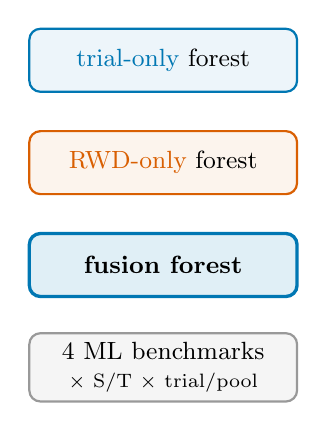
\begin{tikzpicture}[
  cmp/.style={rounded corners=4pt, draw, thick, minimum width=3.4cm,
              minimum height=0.8cm, align=center, font=\small}
]
\node[cmp, draw=rctcol, fill=rctcol!7] (a) at (0,2.2)
  {\textcolor{rctcol}{trial-only} forest};
\node[cmp, draw=rwdcol, fill=rwdcol!7] (b) at (0,0.9)
  {\textcolor{rwdcol}{RWD-only} forest};
\node[cmp, draw=myaccent, very thick, fill=myaccent!12] (c) at (0,-0.4)
  {\textbf{fusion forest}};
\node[cmp, draw=black!40, fill=black!4] (d) at (0,-1.7)
  {4 ML benchmarks\\[-1pt]{\scriptsize $\times$ S/T $\times$ trial/pool}};
\end{tikzpicture}
\end{column}
\end{columns}
\end{frame}

%---------------------------------------------------------
\begin{frame}{Unbiased as the confounding grows}
\vspace{-0.2em}
\begin{center}
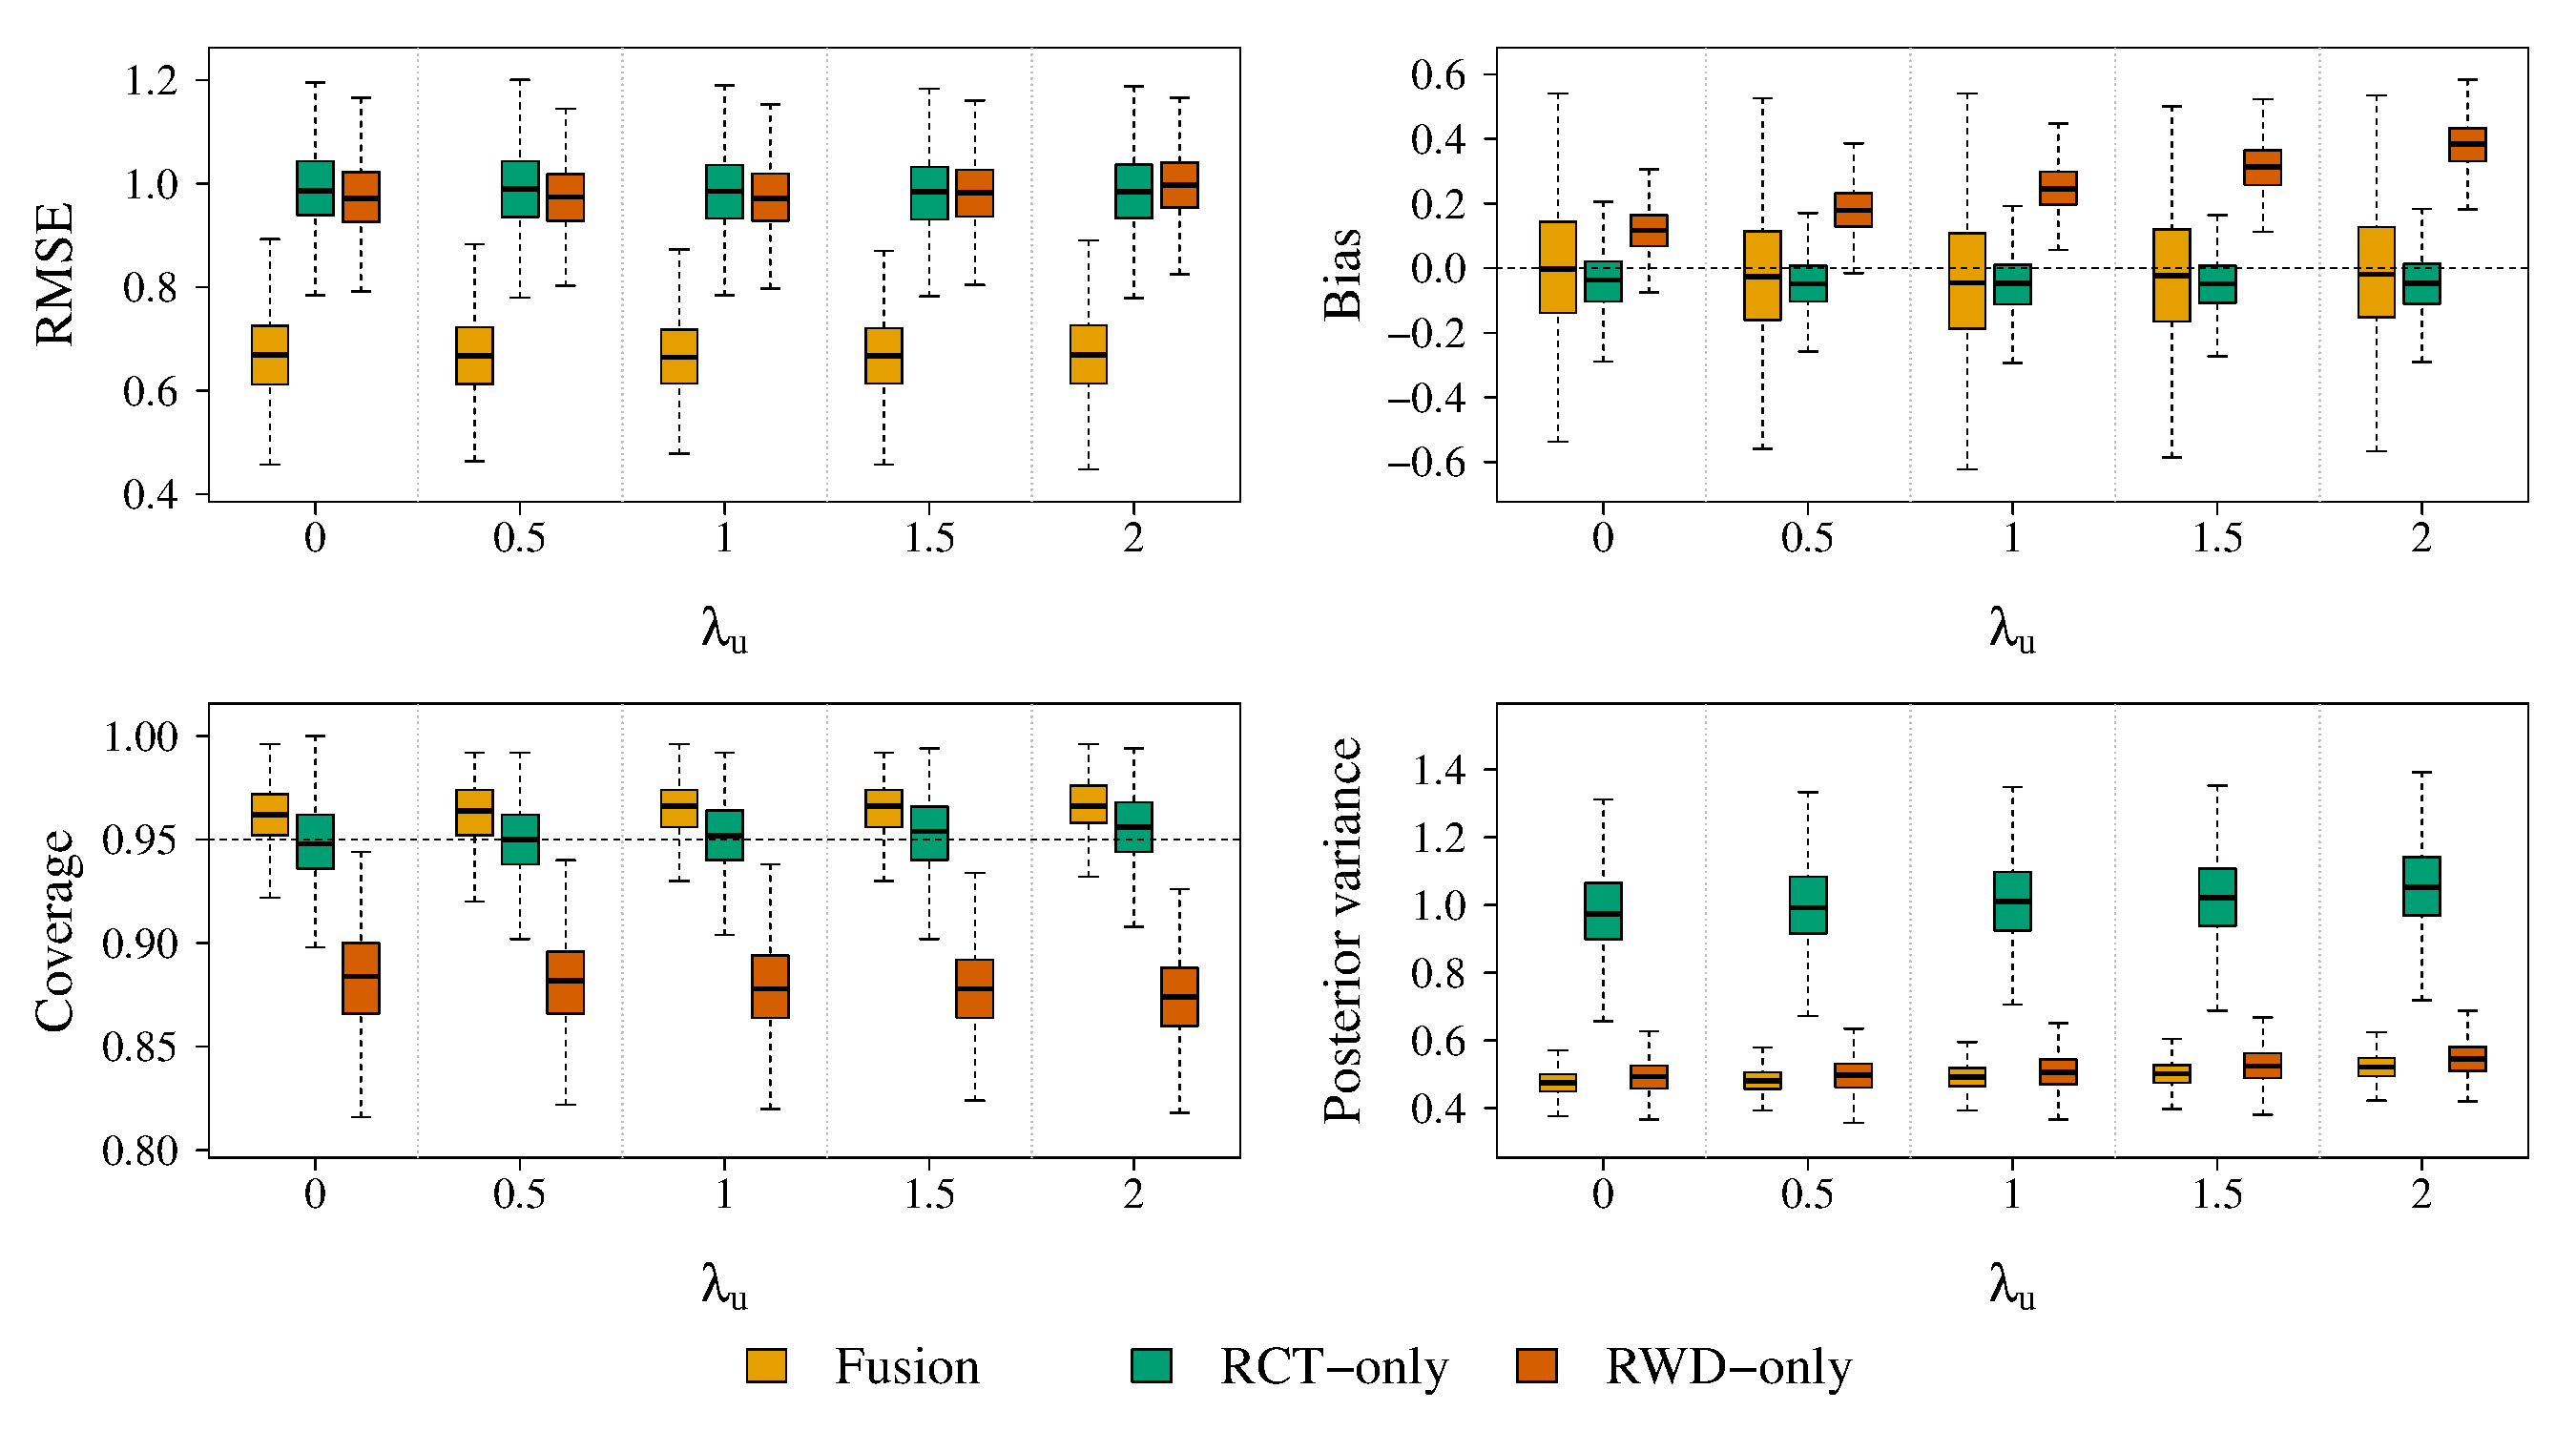
\includegraphics[width=0.78\linewidth]{sim_vary_lambda_u.pdf}
\end{center}
\vspace{-0.3em}
{\footnotesize RWD-only bias grows with $\lambda_u$; fusion stays flat at
\alert{half the posterior variance} of the trial-only fit.}
\end{frame}

%---------------------------------------------------------
\begin{frame}{The gain survives a growing covariate space}
\vspace{-0.2em}
\begin{center}
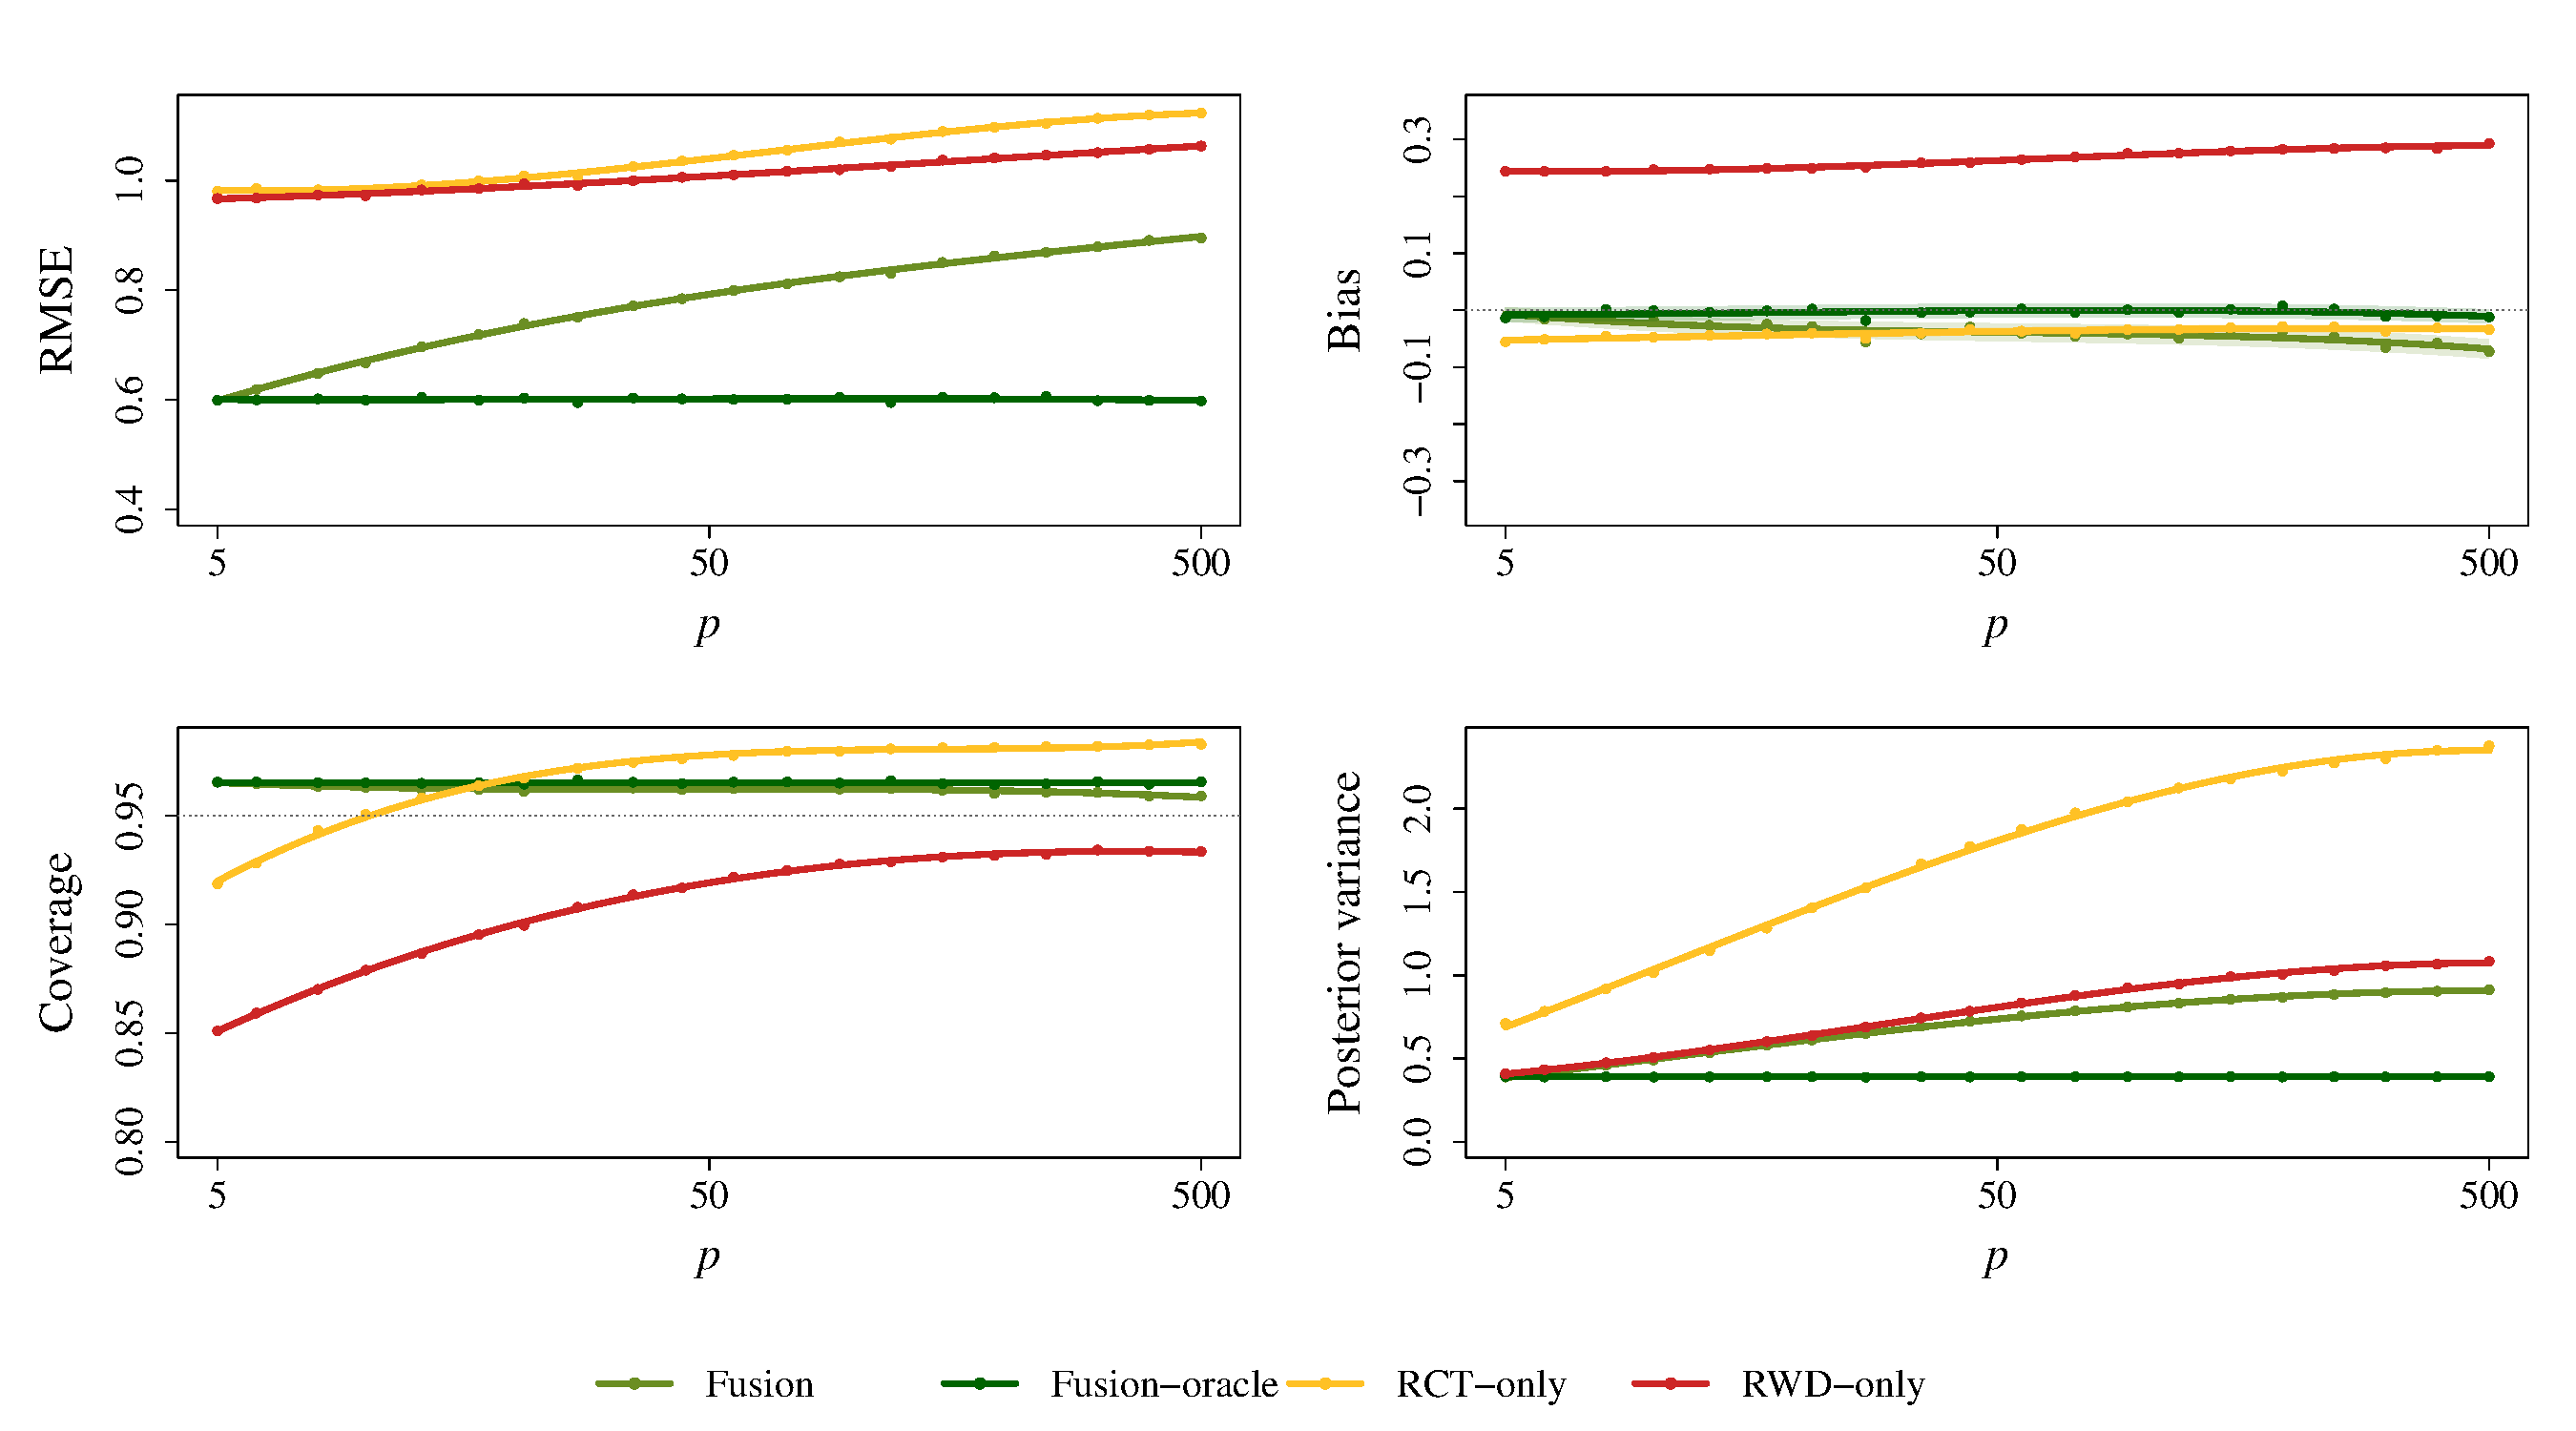
\includegraphics[width=0.76\linewidth]{sim_hd_metrics_vs_p.pdf}
\end{center}
\vspace{-0.3em}
{\footnotesize $p: 5 \to 500$, five active. RMSE ratio to trial-only rises from
$0.68$ to $0.81$ --- \alert{below one throughout}.}
\end{frame}

%---------------------------------------------------------
\begin{frame}{Against flexible machine learning}
\begin{columns}[T,onlytextwidth]
\begin{column}{0.34\textwidth}
\vspace{0.6cm}
Four predictors $\times$ \{S, T\} $\times$ \{trial, pool\}.

\bigskip

None targets a causal contrast; none can separate \cm{taucol}{$\tau$} from
\cm{confcol}{$c$}.

\bigskip

\alert{Only the fusion forest lands in the good corner:} lowest RMSE
\emph{and} nominal coverage.
\end{column}
\begin{column}{0.64\textwidth}
\centering
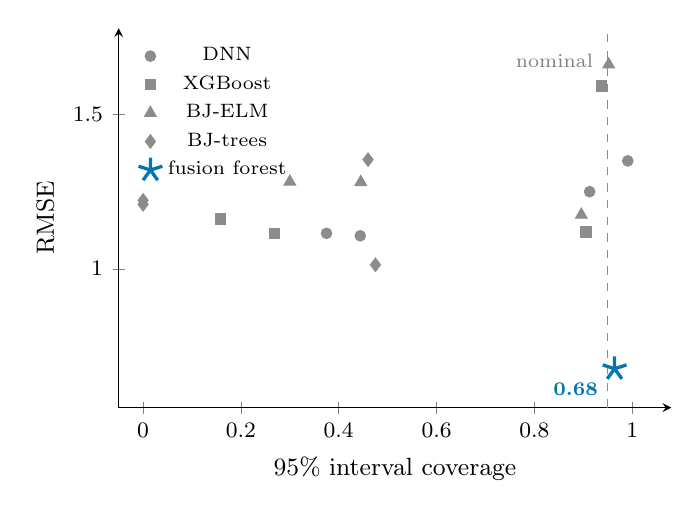
\begin{tikzpicture}
\begin{axis}[
  width=8.6cm, height=6.4cm,
  xlabel={95\% interval coverage}, ylabel={RMSE},
  xmin=-0.05, xmax=1.08, ymin=0.55, ymax=1.78,
  axis lines=left,
  label style={font=\small}, tick label style={font=\footnotesize},
  legend style={font=\scriptsize, draw=none, fill=none,
                at={(0.02,0.98)}, anchor=north west},
  clip=false,
]
\draw[dashed, black!45] (axis cs:0.95,0.55) -- (axis cs:0.95,1.78);
\node[font=\scriptsize, text=black!50, anchor=south east]
  at (axis cs:0.94,1.62) {nominal};

\addplot[only marks, mark=*, mark size=1.9pt, black!45]
  coordinates {(0.375,1.115) (0.913,1.250) (0.444,1.107) (0.991,1.350)};
\addlegendentry{DNN}
\addplot[only marks, mark=square*, mark size=1.9pt, black!45]
  coordinates {(0.158,1.161) (0.937,1.593) (0.269,1.114) (0.905,1.120)};
\addlegendentry{XGBoost}
\addplot[only marks, mark=triangle*, mark size=2.4pt, black!45]
  coordinates {(0.445,1.281) (0.952,1.662) (0.300,1.282) (0.896,1.175)};
\addlegendentry{BJ-ELM}
\addplot[only marks, mark=diamond*, mark size=2.4pt, black!45]
  coordinates {(0.000,1.209) (0.460,1.354) (0.000,1.222) (0.475,1.013)};
\addlegendentry{BJ-trees}

\addplot[only marks, mark=star, mark size=4.5pt, very thick, myaccent]
  coordinates {(0.964,0.676)};
\addlegendentry{fusion forest}
\node[font=\scriptsize\bfseries, text=myaccent, anchor=north east]
  at (axis cs:0.95,0.66) {0.68};
\end{axis}
\end{tikzpicture}
\end{column}
\end{columns}
\end{frame}

%=========================================================
\section{Application}
%=========================================================

%---------------------------------------------------------
\begin{frame}{Combination therapy vs.\ ZDV monotherapy}
\begin{columns}[T,onlytextwidth]
\begin{column}{0.40\textwidth}
\vspace{0.3cm}
Aligned population: men, baseline CD4 $200$--$500$.\\
Six baseline covariates.

\bigskip

\textcolor{rctcol}{ACTG 175}: $n = 1771$, right-censored.\\[3pt]
\textcolor{rwdcol}{MACS}: $n = 373$, interval-censored at annual visits.

\bigskip\bigskip

Average acceleration factor
\[
\widehat{e^{\tau}} = \alert{1.65} \quad [1.43;\, 1.90].
\]
{\footnotesize Trial-only: $1.70$ $[1.51; 1.92]$.}
\end{column}
\begin{column}{0.58\textwidth}
\centering
\vspace{0.1cm}
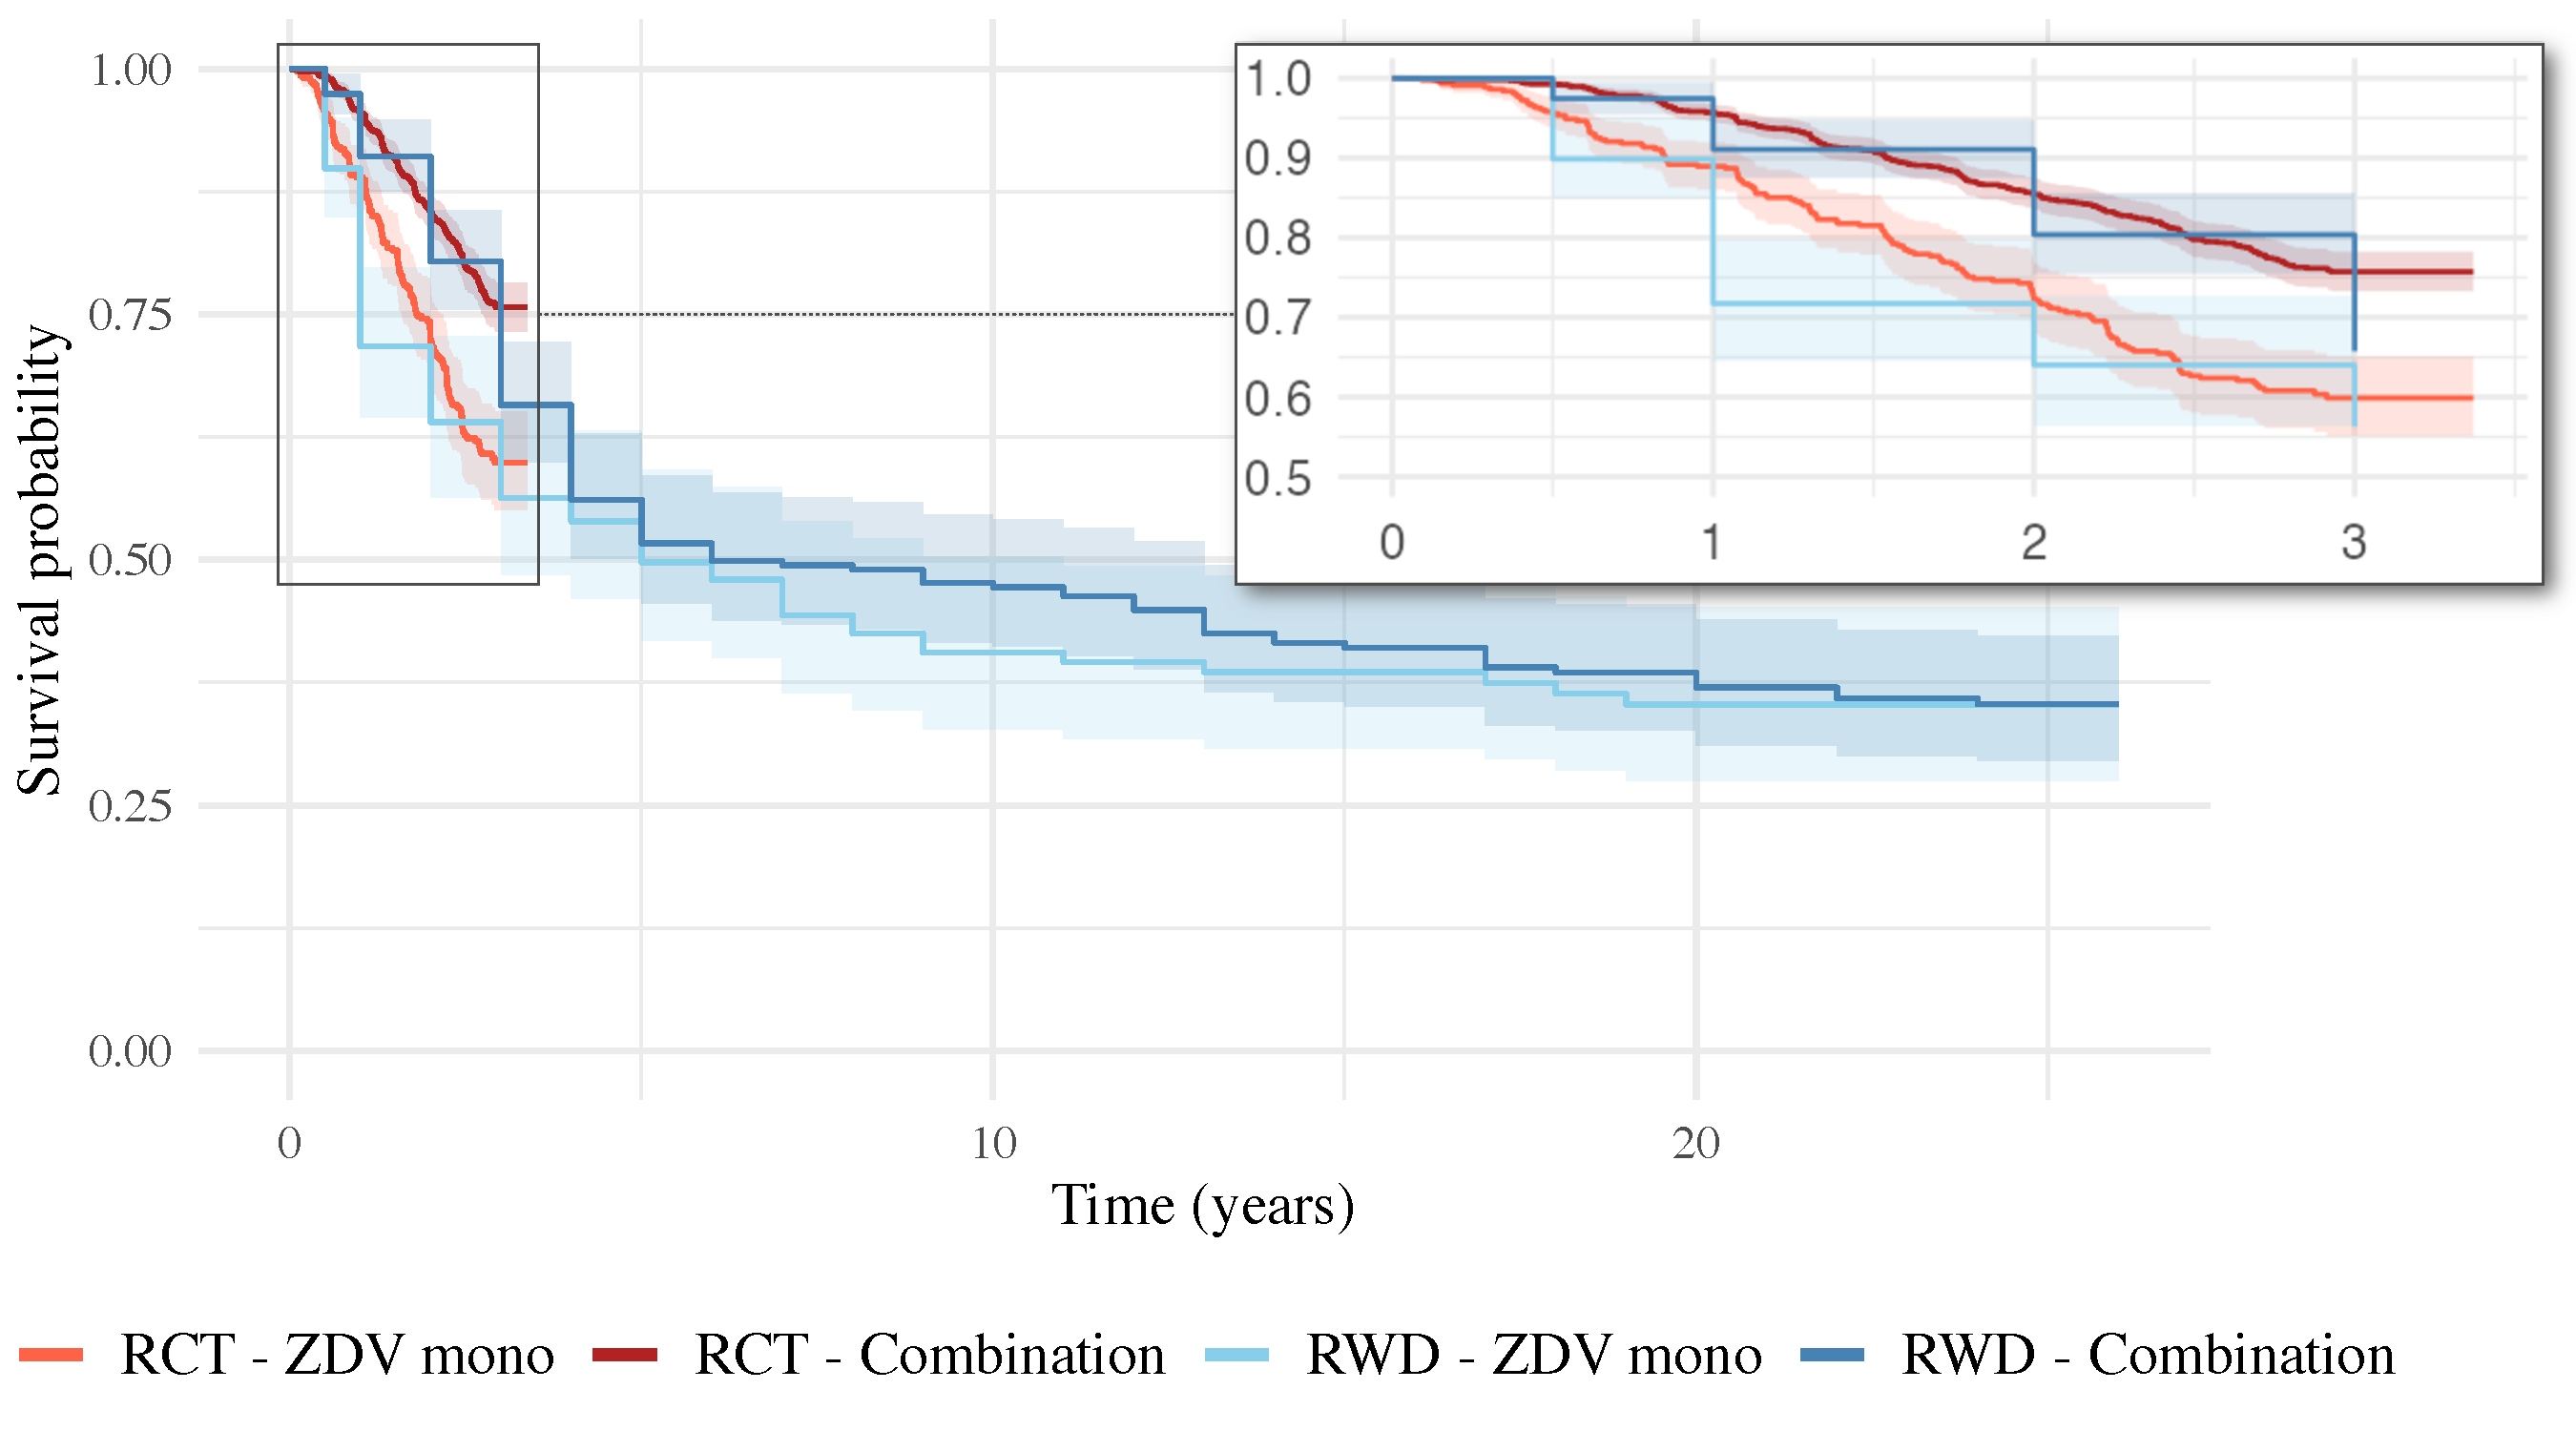
\includegraphics[width=\linewidth]{survival_curves_manuscript.pdf}
\end{column}
\end{columns}
\end{frame}

%---------------------------------------------------------
\begin{frame}{Every patient, with an interval}
\vspace{-0.2em}
\begin{center}
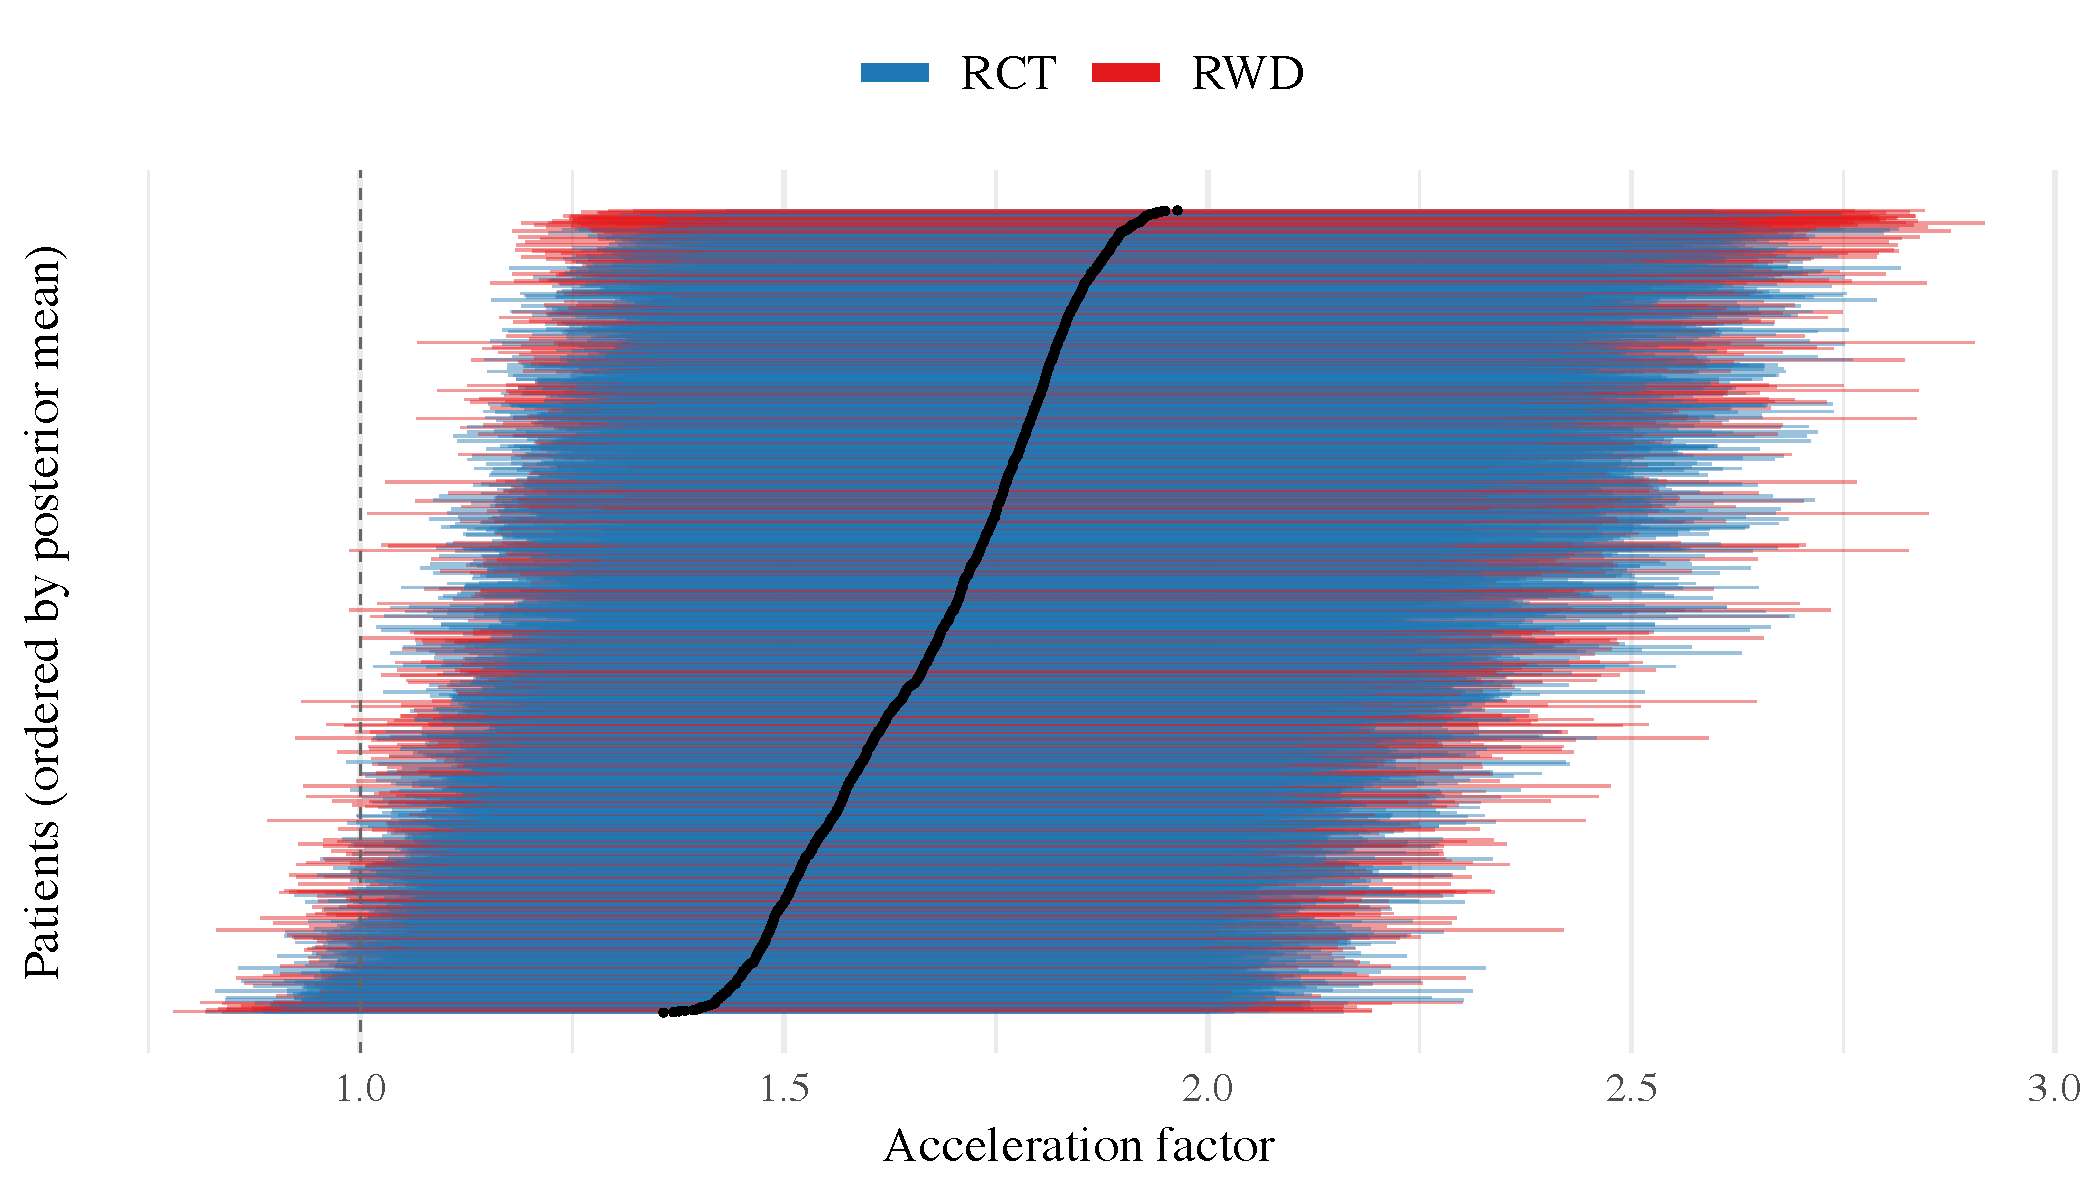
\includegraphics[width=0.70\linewidth]{cate_caterpillar_manuscript.pdf}
\end{center}
\vspace{-0.3em}
{\footnotesize Subject-level acceleration factor, ordered by posterior mean.
Average interval width falls from $3.16$ to $1.21$: \alert{a $62\%$ reduction}
over the trial alone.}
\end{frame}

%---------------------------------------------------------
\begin{frame}{From inconclusive to near-certain}
\begin{columns}[T,onlytextwidth]
\begin{column}{0.36\textwidth}
\vspace{0.9cm}
Posterior probability of benefit,\\ $\p(\tau(x_i) > 0 \mid \text{data})$,
over the \emph{trial} population.

\bigskip

The trial alone leaves a quarter of patients inconclusive.

\bigskip

\alert{The fusion finds benefit for nearly everyone} --- with a slightly
\emph{smaller} average effect.
\end{column}
\begin{column}{0.62\textwidth}
\centering
\vspace{0.4cm}
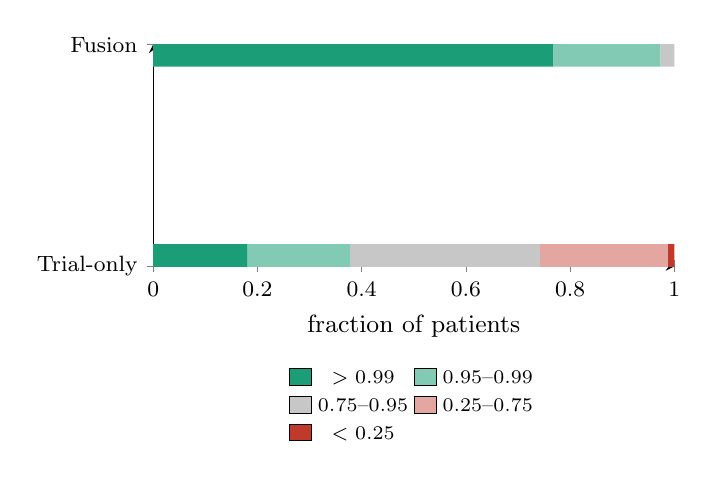
\begin{tikzpicture}
\begin{axis}[
  xbar stacked,
  width=8.2cm, height=4.4cm,
  xmin=0, xmax=1,
  xlabel={fraction of patients},
  symbolic y coords={Trial-only, Fusion},
  ytick=data,
  axis lines=left,
  bar width=16pt,
  label style={font=\small}, tick label style={font=\footnotesize},
  legend style={font=\scriptsize, draw=none, fill=none, legend columns=2,
                at={(0.5,-0.42)}, anchor=north},
]
\addplot[fill=taucol, draw=none]        coordinates {(0.767,Fusion) (0.180,Trial-only)};
\addlegendentry{$>0.99$}
\addplot[fill=taucol!55, draw=none]     coordinates {(0.206,Fusion) (0.198,Trial-only)};
\addlegendentry{$0.95$--$0.99$}
\addplot[fill=black!22, draw=none]      coordinates {(0.028,Fusion) (0.364,Trial-only)};
\addlegendentry{$0.75$--$0.95$}
\addplot[fill=confcol!45, draw=none]    coordinates {(0.000,Fusion) (0.245,Trial-only)};
\addlegendentry{$0.25$--$0.75$}
\addplot[fill=confcol, draw=none]       coordinates {(0.000,Fusion) (0.014,Trial-only)};
\addlegendentry{$<0.25$}
\end{axis}
\end{tikzpicture}
\end{column}
\end{columns}
\end{frame}

%---------------------------------------------------------
\begin{frame}{Who benefits most?}
\vspace{0.1cm}
\begin{center}
\definecolor{splitfill}{RGB}{230,244,250}
\resizebox{0.86\textwidth}{!}{%
\begin{tikzpicture}[
  every node/.style = {align=center, font=\footnotesize},
  splitn/.style     = {draw, rounded corners=2pt, fill=splitfill,
                       minimum width=1.15cm, minimum height=0.55cm,
                       inner sep=2.5pt},
  leafn/.style      = {draw, rounded corners=2pt, fill=white,
                       minimum width=1.45cm, minimum height=0.85cm,
                       inner sep=3pt, font=\scriptsize},
  elabel/.style     = {midway, fill=white, inner sep=3pt, font=\scriptsize},
  edgeln/.style     = {draw=black!55, thick}]

  \node[splitn] (root)  at ( 0.35, 4.7) {CD8};
  \node[splitn] (mid1)  at (-3.00, 3.4) {CD8};
  \node[splitn] (mid2)  at ( 3.70, 3.4) {CD8};
  \node[splitn] (raceA) at (-4.50, 1.9) {race};
  \node[splitn] (raceB) at ( 1.70, 1.9) {race};
  \node[splitn] (raceC) at ( 5.70, 1.9) {race};

  \node[leafn] (L1) at (-5.4, 0) {$1.45$\\$n = 124$};
  \node[leafn] (L2) at (-3.6, 0) {$1.51$\\$n = 381$};
  \node[leafn] (L3) at (-1.4, 0) {$1.60$\\$n = 330$};
  \node[leafn] (L4) at ( 0.8, 0) {$1.65$\\$n = 107$};
  \node[leafn] (L5) at ( 2.6, 0) {$1.72$\\$n = 425$};
  \node[leafn] (L6) at ( 4.8, 0) {$1.76$\\$n = 178$};
  \node[leafn] (L7) at ( 6.6, 0) {$1.83$\\$n = 599$};

  \draw[edgeln] (root) -- (mid1)  node[elabel] {$\le 800$};
  \draw[edgeln] (root) -- (mid2)  node[elabel] {$> 800$};
  \draw[edgeln] (mid1) -- (raceA) node[elabel] {$\le 650$};
  \draw[edgeln] (mid1) -- (L3)    node[elabel] {$> 650$};
  \draw[edgeln] (mid2) -- (raceB) node[elabel] {$\le 1065$};
  \draw[edgeln] (mid2) -- (raceC) node[elabel] {$> 1065$};
  \draw[edgeln] (raceA) -- (L1) node[elabel] {non-white};
  \draw[edgeln] (raceA) -- (L2) node[elabel] {white};
  \draw[edgeln] (raceB) -- (L4) node[elabel] {non-white};
  \draw[edgeln] (raceB) -- (L5) node[elabel] {white};
  \draw[edgeln] (raceC) -- (L6) node[elabel] {non-white};
  \draw[edgeln] (raceC) -- (L7) node[elabel] {white};
\end{tikzpicture}}
\end{center}

\vspace{0.2cm}
{\footnotesize Posterior projection of \cm{taucol}{$\tau$} onto a depth-three
tree. Only CD8 and race enter; \alert{every leaf exceeds $1.4$}.}
\end{frame}

%=========================================================
\section{Wrap-up}
%=========================================================

%---------------------------------------------------------
\begin{frame}{Take-aways}
\begin{itemize}
  \item \textbf{Trade one assumption for another.} Give up unconfoundedness in
        the real-world data; keep transportability of the effect. The
        confounding function absorbs the rest.
  \vspace{0.7cm}
  \item \textbf{Put the borrowing in the prior.} A forest per causal component,
        each regularised for its role --- shared baseline, mean-zero deviation,
        shrunken confounding.
  \vspace{0.7cm}
  \item \textbf{It pays off.} Unbiased under confounding, half the posterior
        variance of a trial-only analysis, and benefit established for nearly
        every HIV patient where the trial alone was inconclusive.
\end{itemize}
\end{frame}

%---------------------------------------------------------
\begin{frame}{Thanks for your attention!}
\vspace{0.4cm}
\begin{columns}[T,onlytextwidth]

\begin{column}{0.33\textwidth}
\centering
\begin{minipage}[t][2.6cm][c]{\linewidth}\centering

\begin{tikzpicture}[scale=0.95]
\fill[white] (0, 0) rectangle (1.6, 2.2);
\draw[myaccent, thick] (0, 0) rectangle (1.6, 2.2);
\fill[myaccent] (0, 1.85) rectangle (1.6, 2.2);
\draw[white, line width=0.8pt] (0.2, 2.025) -- (1.4, 2.025);
\foreach \y in {1.6, 1.4, 1.2, 1.0, 0.8, 0.6, 0.4} {
  \draw[gray!50, thick] (0.15, \y) -- (1.45, \y);
}
\end{tikzpicture}
\end{minipage}

\bigskip

\begin{minipage}[t][2.0cm][t]{\linewidth}\centering
\textbf{Paper}\\[4pt]
{\footnotesize Preprint on arXiv.}
\end{minipage}
\end{column}

\begin{column}{0.33\textwidth}
\centering
\begin{minipage}[t][2.6cm][c]{\linewidth}\centering

\includegraphics[height=2.5cm]{../../sticker/FusionForests_hex.png}
\end{minipage}

\bigskip

\begin{minipage}[t][2.0cm][t]{\linewidth}\centering
\textbf{R package} \texttt{FusionForests}\\[4pt]
{\footnotesize on GitHub; CRAN planned.}
\end{minipage}
\end{column}

\begin{column}{0.33\textwidth}
\centering
\begin{minipage}[t][2.6cm][c]{\linewidth}\centering
\qrcode[height=2.5cm]{https://tijn-jacobs.github.io/}
\end{minipage}

\bigskip

\begin{minipage}[t][2.0cm][t]{\linewidth}\centering
\textbf{Stay up to date}\\[4pt]
{\footnotesize \texttt{tijn-jacobs.github.io}}
\end{minipage}
\end{column}

\end{columns}
\end{frame}

%---------------------------------------------------------
\begin{frame}{References}
\footnotesize
\begin{itemize}
  \item Chipman, H.A., George, E.I., McCulloch, R.E. (2010). BART: Bayesian
        additive regression trees. \emph{Annals of Applied Statistics}, 4(1), 266--298.
  \item Hahn, P.R., Murray, J.S., Carvalho, C.M. (2020). Bayesian regression tree
        models for causal inference. \emph{Bayesian Analysis}, 15(3), 965--1056.
  \item Robins, J.M. (2000). Sensitivity analysis for selection bias and
        unmeasured confounding. \emph{IMA Volumes in Mathematics}, 116, 1--94.
  \item Neuenschwander, B., et al. (2010). Summarizing historical information on
        controls in clinical trials. \emph{Clinical Trials}, 7(1), 5--18.
  \item Teh, Y.W., Jordan, M.I., Beal, M.J., Blei, D.M. (2006). Hierarchical
        Dirichlet processes. \emph{JASA}, 101(476), 1566--1581.
  \item Brathovde, M., Putter, H., Valberg, M., Post, R.A.J. (2024). The causal
        interpretation of acceleration factors. \emph{arXiv:2409.01983}.
\end{itemize}

\vfill

\begin{columns}[c,onlytextwidth]
\begin{column}{0.68\textwidth}
\tiny
This work was supported by the European Research Council (grant 101074802) and
the SURF Cooperative (grant EINF-18803). Views and opinions expressed are those
of the authors only and do not necessarily reflect those of the European Union
or the European Research Council Executive Agency. Neither the European Union
nor the granting authority can be held responsible for them.
\end{column}
\begin{column}{0.30\textwidth}
\centering
\IfFileExists{figures/EU-funding.jpg}
  {\includegraphics[width=0.7\linewidth]{figures/EU-funding.jpg}}{}
\end{column}
\end{columns}
\end{frame}

%=========================================================
\appendix
\section{Backup}
%=========================================================

%---------------------------------------------------------
\begin{frame}{Assumptions in full}
\begin{enumerate}\setlength\itemsep{0.4em}
  \item \textbf{Consistency.} $A = a \Rightarrow T = T(a)$, $\mathcal{C} = \mathcal{C}(a)$.
  \item \textbf{Unconfoundedness of the RCT.} $T(a) \indep A \mid X,\, S = 1$.
  \item \textbf{Positivity.} $0 < \p(A = 1 \mid X = x,\, S = s) < 1$.
  \item \textbf{Cross-source transportability.}
        $\E[\log T(1) - \log T(0) \mid X, S = 1] = \E[\log T(1) - \log T(0) \mid X, S = 0]$.
  \item \textbf{Conditionally non-informative censoring.}
        $T(a) \indep \mathcal{C}(a) \mid X,\, A,\, S$.
\end{enumerate}

\bigskip

{\footnotesize Assumptions 1, 3 and 5 are standard. Assumption 5 enters only the
likelihood and the data augmentation, never the identification argument --- which
is why interval censoring costs nothing causally.}
\end{frame}

%---------------------------------------------------------
\begin{frame}{The confounding function}
\[
c(x) \;=\;
\underbrace{\E[\log T \mid x, A = 1, S = 0] - \E[\log T \mid x, A = 0, S = 0]}_{\text{observed RWD contrast}}
\;-\; \cm{taucol}{\tau(x)}
\]

\bigskip

\begin{itemize}
  \item Introduced as a sensitivity-analysis device within a single study
        (Robins, 2000).
  \item Here it is a \emph{fitted} object: the trial identifies
        \cm{taucol}{$\tau$}, so the RWD identifies \cm{confcol}{$c$}.
  \item Shrunk towards a constant: $(\alpha_c, \beta_c) = (0.25, 3)$, $J_c = 50$.
\end{itemize}
\end{frame}

%---------------------------------------------------------
\begin{frame}{Full model}
\vspace{-0.3cm}
\begin{align*}
\log T_i &= \cm{basecol}{m_0^{\mathrm{sh}}(X_i)} + (1 - S_i)\, \cm{devcol}{d(X_i)}
           + A_i\, \cm{taucol}{\tau(X_i)} + (1 - S_i) A_i\, \cm{confcol}{c(X_i)} + \varepsilon_i, \\[2pt]
\cm{basecol}{m_0^{\mathrm{sh}}} &\sim \mathrm{BART}(200,\, k_{\mathrm{sh}},\, 0.95,\, 2), \\
\cm{devcol}{d} &\sim \mathrm{BART}(50,\, k_d,\, 0.95,\, 2), \\
\cm{taucol}{\tau} &\sim \mathrm{BART}(100,\, k_\tau,\, 0.95,\, 3), \\
\cm{confcol}{c} &\sim \mathrm{BART}(50,\, k_c,\, 0.25,\, 3), \\[2pt]
\varepsilon_i \mid S_i = s &\sim \textstyle\int \sigma_s^{-1} \phi\bigl((w - \theta)/\sigma_s\bigr)\, dG_s(\theta), \\
G_s &= \textstyle\sum_k \pi_{sk}\, \delta_{\theta_k^* - \mu_s}, \\
G_s^* \mid G^*, M_s &\sim \mathrm{DP}(M_s, G^*), \qquad
G^* \mid \gamma \sim \mathrm{DP}(\gamma, H), \quad H = \N(0, \sigma_\theta^2), \\
\gamma &\sim \mathrm{Gamma}(a_\gamma, b_\gamma), \qquad
M_s \sim \mathrm{Gamma}(a_M, b_M), \qquad
\sigma_s^2 \sim \nu\lambda / \chi^2_\nu.
\end{align*}
\end{frame}

%---------------------------------------------------------
\begin{frame}{Full comparison with machine-learning alternatives}
\centering
\scriptsize
\renewcommand{\arraystretch}{0.85}
\begin{tabular}{@{}lll rrrr@{}}
\toprule
Method & Source & Learner & RMSE & Bias & Coverage & Width \\
\midrule
Bayesian fusion forest & Both & --- & $\mathbf{0.676}$ & $\mathbf{-0.026}$ & 0.964 & 2.82 \\
\midrule
DNN     & Trial & S & 1.115 & $-0.185$ & 0.375 & 0.95 \\
        &       & T & 1.250 & $-0.247$ & 0.913 & 3.73 \\
        & Pool  & S & 1.107 & 0.105 & 0.444 & 0.99 \\
        &       & T & 1.350 & 0.137 & 0.991 & 4.92 \\
\addlinespace
XGBoost & Trial & S & 1.161 & $-0.038$ & 0.158 & 0.40 \\
        &       & T & 1.593 & $-0.075$ & 0.937 & 4.95 \\
        & Pool  & S & 1.114 & 0.151 & 0.269 & 0.64 \\
        &       & T & 1.120 & 0.306 & 0.905 & 3.27 \\
\addlinespace
BJ-ELM  & Trial & S & 1.281 & $-0.068$ & 0.445 & 1.42 \\
        &       & T & 1.662 & 0.393 & 0.952 & 5.97 \\
        & Pool  & S & 1.282 & 0.309 & 0.300 & 0.90 \\
        &       & T & 1.175 & 0.472 & 0.896 & 3.34 \\
\addlinespace
BJ-trees& Trial & S & 1.209 & $-0.040$ & 0.000 & 0.00 \\
        &       & T & 1.354 & $-0.054$ & 0.460 & 1.73 \\
        & Pool  & S & 1.222 & 0.028 & 0.000 & 0.00 \\
        &       & T & 1.013 & 0.343 & 0.475 & 1.25 \\
\bottomrule
\end{tabular}

\vspace{0.3cm}
{\scriptsize $\lambda_d = \lambda_u = 1$; both sources right-censored at
$\approx 35\%$; 1000 replications.}
\end{frame}

%---------------------------------------------------------
\begin{frame}{How do the two baselines differ?}
\begin{columns}[T,onlytextwidth]
\begin{column}{0.46\textwidth}
\vspace{0.4cm}
Linear projection of the deviation forest \cm{devcol}{$d(x)$}:

\bigskip

\begin{itemize}
  \item Intercept $1.70$ $[1.31; 2.10]$.
  \item Prior ART years $0.27$ $[-0.01; 0.55]$.
  \item Age, CD4, CD8, year, race: all near zero.
\end{itemize}

\bigskip

\alert{The gap is essentially a constant shift} --- the cohort baseline sits
well above the trial.
\end{column}
\begin{column}{0.52\textwidth}
\centering
\vspace{0.2cm}
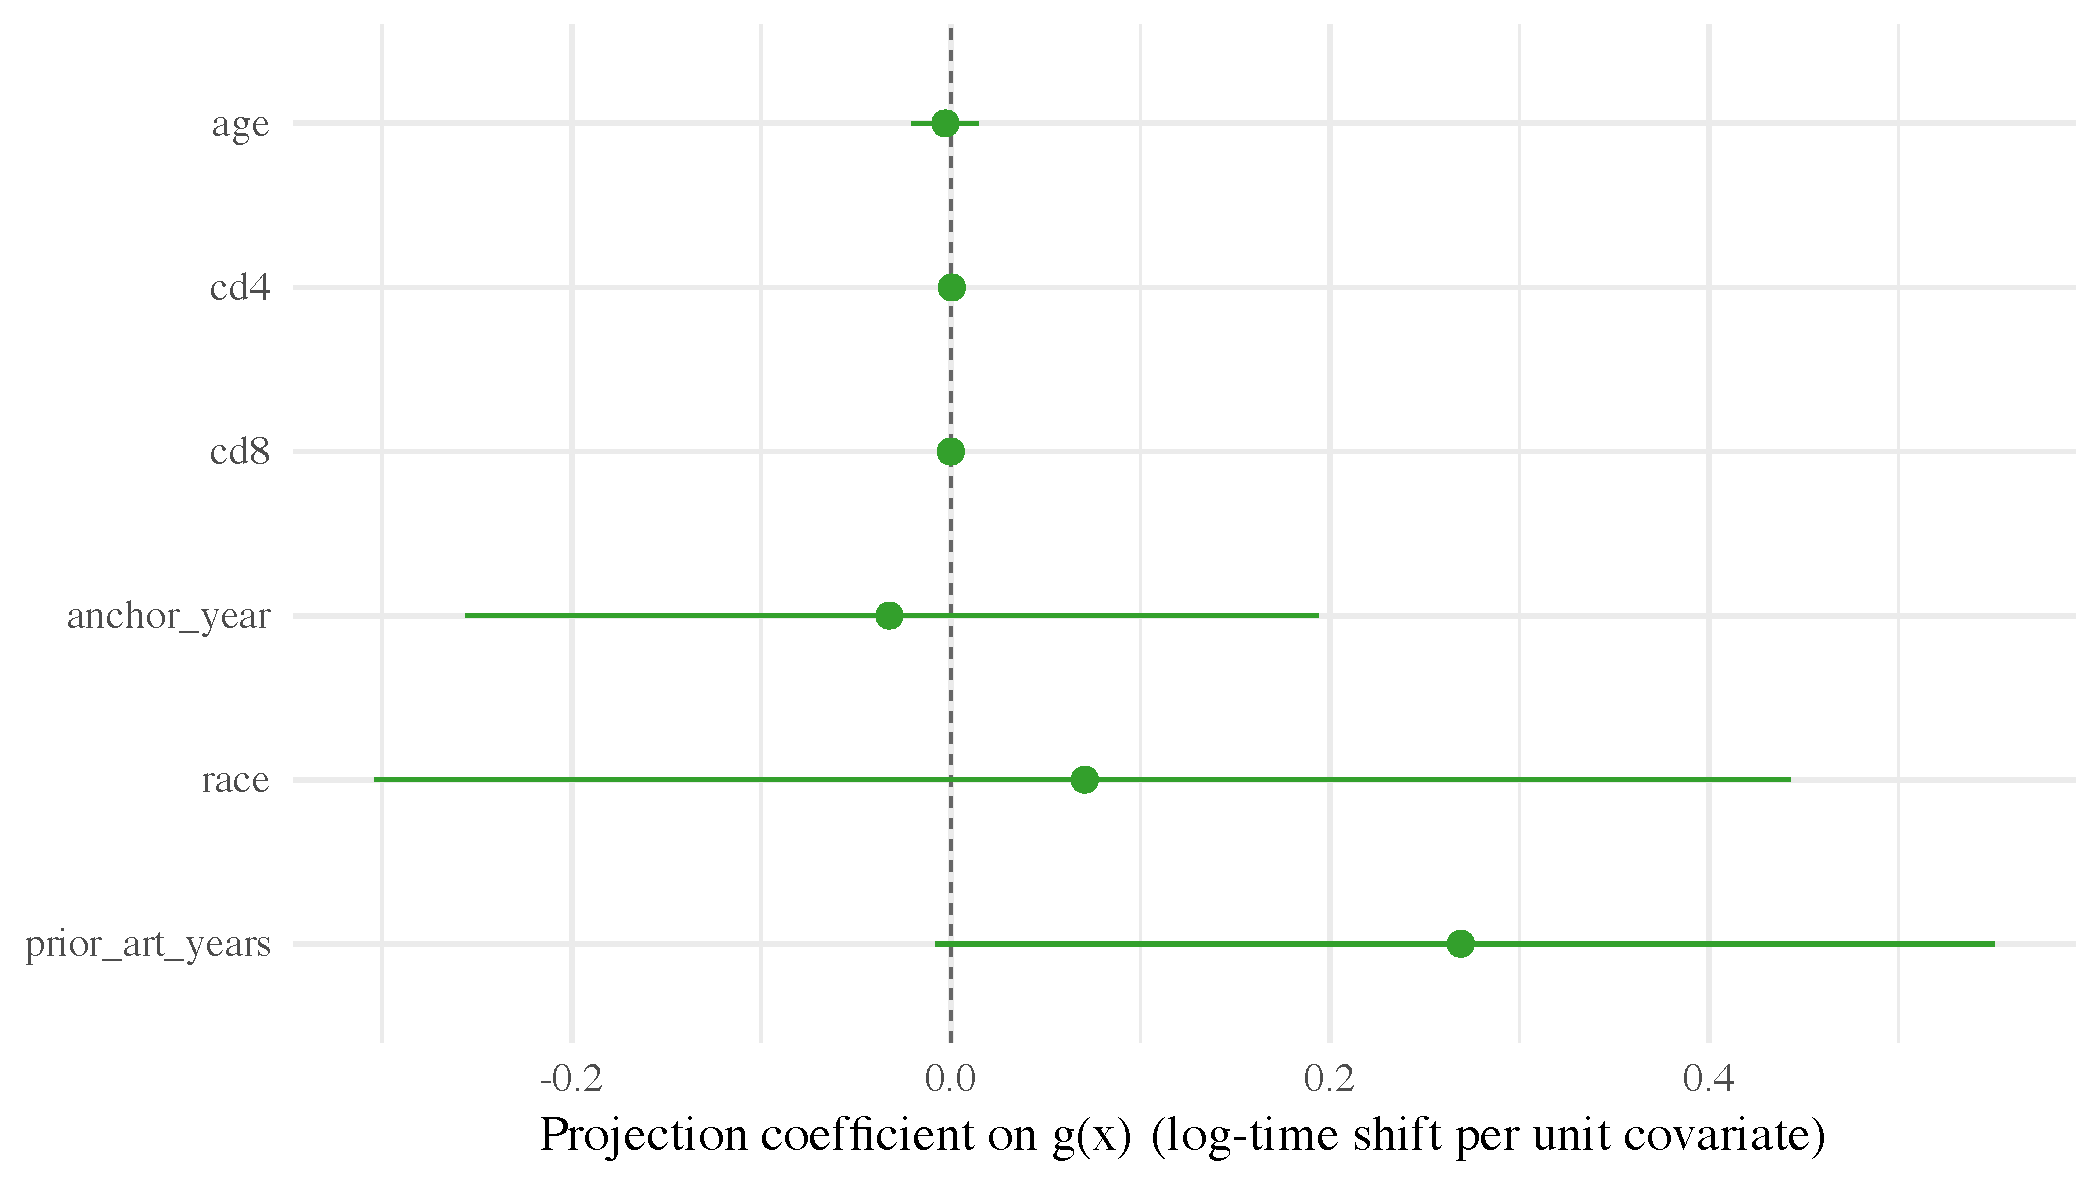
\includegraphics[width=\linewidth]{projection_deviation_manuscript.pdf}
\end{column}
\end{columns}
\end{frame}

%---------------------------------------------------------
\begin{frame}{Between-source heterogeneity $\lambda_d$}
\vspace{-0.2em}
\begin{center}
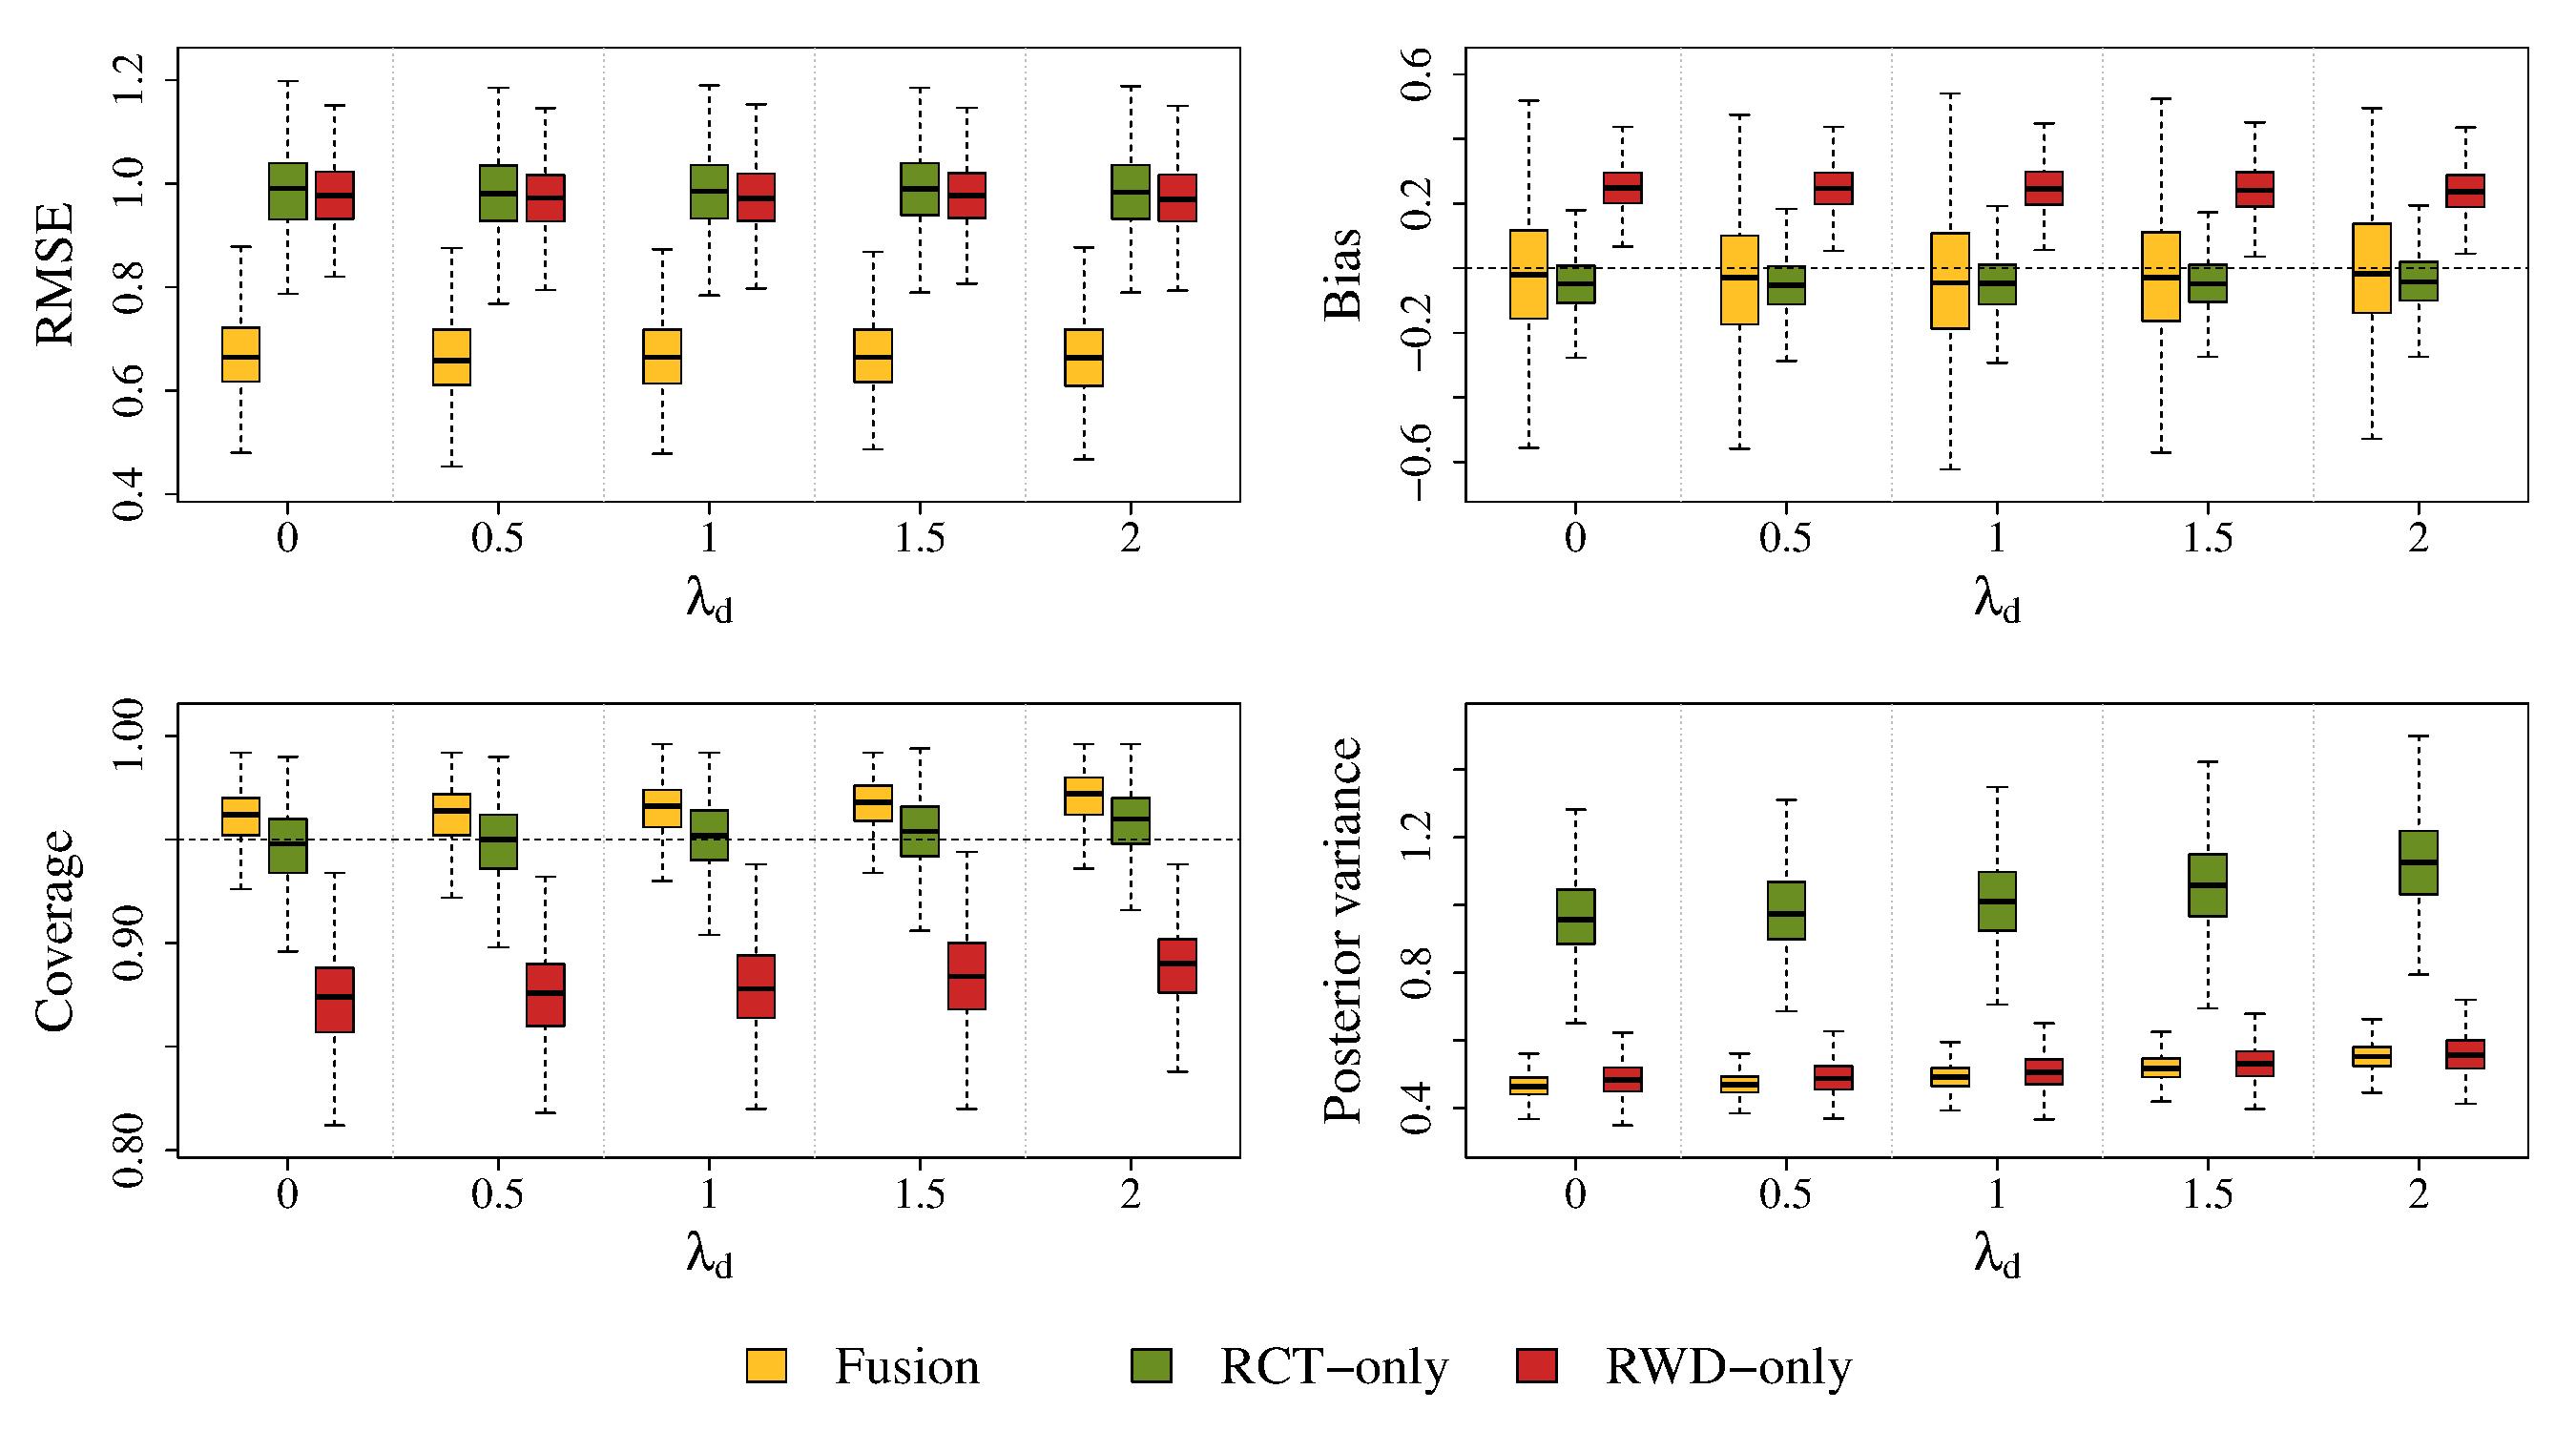
\includegraphics[width=0.78\linewidth]{sim_vary_lambda_d.pdf}
\end{center}
\vspace{-0.3em}
{\footnotesize All three estimators are flat in $\lambda_d$: the deviation
forest absorbs the gap.}
\end{frame}

\end{document}
